\documentclass{ieeeaccess}
\usepackage{cite}
\usepackage{amsmath,amssymb,amsfonts}
\usepackage{algorithmic}
\usepackage{graphicx}
\usepackage{stfloats}
\usepackage{subfigure}
\usepackage{float}
\usepackage{multirow}
\usepackage{multicol}
\usepackage{enumitem}
\usepackage{xcolor}
\usepackage{romannum}% for approach #1 and #2




\usepackage{textcomp}
\def\BibTeX{{\rm B\kern-.05em{\sc i\kern-.025em b}\kern-.08em
    T\kern-.1667em\lower.7ex\hbox{E}\kern-.125emX}}
\begin{document}
\history{Date of publication xxxx 00, 0000, date of current version xxxx 00, 0000.}
\doi{10.1109/ACCESS.2017.DOI}

\title{SENext: Squeeze-and-ExcitationNext for Single Image Super-Resolution}
\author{\uppercase{Wazir Muhammad}\authorrefmark{1}, \IEEEmembership{Graduate Student Member, IEEE},
\uppercase{SUPAVADEE ARAMVITH}\authorrefmark{2},\IEEEmembership{Senior Member, IEEE}, AND
\uppercase{Takao Onoye }\authorrefmark{3},
\IEEEmembership{Senior Member, IEEE}}
\address[1]{Department of Electrical Engineering, Chulalongkorn University, Bangkok 10330, Thailand}
\address[2]{Multimedia Data Analytics and Processing Unit, Department of Electrical Engineering, Faculty of Engineering, Chulalongkorn University, Bangkok 10330, Thailand}
\address[3]{Graduate School of Information Science and Technology, Osaka University, 1-5 Yamada-Oka, Suita, 565-0871 Japan}
\tfootnote{This research is funded by the Second Century Fund (C2F) Chulalongkorn University, Electrical Engineering Department Chulalongkorn University Bangkok, Thailand. This research is also funded by Thailand Science Research and Innovation Fund Chulalongkorn University (CU\textunderscore FRB65\textunderscore ind (9)\textunderscore 157\textunderscore 21\textunderscore 23), The NSRF via the Program Management Unit for Human Resources \& Institutional Development, Research and Innovation [grant number B$04G640053$] and also funded by Thailand Science research and Innovation Fund Chulalongkorn University (IND$66210019$).} \markboth
{Author \headeretal: Preparation of Papers for IEEE TRANSACTIONS and JOURNALS}
{Author \headeretal: Preparation of Papers for IEEE TRANSACTIONS and JOURNALS}

\corresp{Corresponding author:  Supavadee Aramvith (supavadee.a@chula.ac.th).}

\begin{abstract}
Recent research on image and video processing using convolutional neural networks has shown remarkable improvements, especially in the area of single image super-resolution(SISR). The primary target of SISR is to recover the visually appealing high-resolution (HR) output image from the original degraded low-resolution (LR) input image. However, most recent convolutional neural networks (CNNs)-based image super-resolution frameworks often used a deeper and broader network architecture that requires a sizeable computational resource, risk of overfitting, increases computational complexity, and more memory consumption, as well as takes more processing time during the evaluations. To address these issues, we have presented a Squeeze-and-ExcitationNext for Single Image Super-Resolution approach, known as SENext. In brief, the squeeze-and-excitation blocks (SEB) are used in our network architecture with a view to reduce the computational cost and adopt the channel-wise feature mappings to recalibrate the features adaptively. Furthermore, local, sub-local, and global skip connections are employed between each SEB to enable the feature reusability and stabilize training convergence smoothly. Instead of hand-designed bicubic upsampling at pre-processing step, we have performed post-upsampling at the later stage to reconstruct the high-resolution image. Extensive quantitative and qualitative experiments are performed on the benchmark test dataset, including Set5, Set14, BSDS100, Urban100, and Manga109. These experimental evaluations validate the superiority of the SENext over other deep CNN image SR methods in terms of PSNR/SSIM, FLOPs, Number of parameters, processing speed, and visually pleasing effect.
\end{abstract}

\begin{keywords}
Convolutional Neural Networks, LeakyReLU activation function, Squeeze-and-excitation block.
\end{keywords}

\titlepgskip=-15pt

\maketitle

\section{Introduction}
\label{sec:introduction}
\PARstart{O}{ne} of the most significant research area in convolutional neural network-based image processing is a single image super-resolution (SISR). SISR function is to reconstruct the visually appealing high-resolution (HR) output image from the input low-resolution (LR) image.  However, SISR is still a difficult task and is considered as an inverse and ill-posed problems and numerous algorithms [1-5] have been discussed. Although these algorithms have improved the condition of LR image, but performance is not satisfactory and has more computational complexity. Recently, deep convolutional neural networks (CNNs) captured the market of image SR, and the research community shifted from the old hand-designed approach to a new deep CNN-based approach. Initially, Dong \textit{et al.} recovered a new idea and proposed a shallow-type super-resolution convolutional neural network (SRCNN) [6] architecture to reconstruct a better HR image from the bicubic interpolated generated LR input image. SRCNN [6] consists of three basic types of CNN layers: patch extraction, mapping, and reconstructed layers. Apart from the success of SRCNN [6] in the image super-resolution, it has various limitations, containing slow training speed, weak real-time restoration, bicubic interpolation as a pre-processing stage, and large convolution kernels used during the model design. In response to these problems, the same author has proposed the revised version of SRCNN [6] and replaced the bicubic interpolation with a learnable upsampling transposed convolutional layer to accomplish post-upsampling SR named  fast super-resolution CNN (FSRCNN) [7]. Furthermore, larger kernel sizes of SRCNN [6] are replaced with smaller kernels to boost up training efficiency and reconstruction quality. FSRCNN [7] improved the performance and decreased the computational cost compared to the previous SRCNN [6]. The main drawback of FSRCNN [7] is the capacity of a network is limited. Kim \textit{et al.} first time follow the idea of  visual geometry group network (VGGNet) [8] to proposed a Very Deep Super-Resolution (VDSR) [9], which pushed up the network and serially stacking multiple layers up to 20. The performance of the VDSR [9] model significantly improved over previous models. This method suggested that deeper model architecture is the better and to increase the visual quality of the HR image. Initially, a sub-pixel layer-based model used in image super-resolution was suggested by Shi \textit{et al.} and named as an efficient sub-pixel convolutional neural network (ESPCN) [10] to decrease the computational burden as well as revise the upscaling process. In this approach, the authors change the pre-stage upscaling bicubic operator with a sub-pixel convolution layer, and features are recovered from the original low-dimensional space to decrease the model processing time during the training as well as testing. Kim \textit{et al.} suggested a new way of architecture known as deeply-recursive convolutional network (DRCN) [11]  and replaced the serial way of a combination of CNN layers with a recursive manner. This architecture's main benefit is to constantly maintaining network parameters, but the training convergence process is too slow.

Additionally, to obtain better reconstruction performance, the SR models used the concept of a deeper model and stacking the side layer by the side. In some cases, the model depth increases up to 100 layers observed [12]. A super-resolution model's performance can be enhanced by increasing its spatial depth, but doing so will suffer a significant computational expense and memory usage. Furthermore, deep CNN-based methods employed the bicubic pre-processing operation as shown in Figure 1, such as SRCNN [6], VDSR [9], and DRCN [11]. The main issue with these approaches having a more computational cost and reconstructing HR images having blurry results. To lessen the computational complexity and increase the processing speed of image SR models inspired by the Squeeze-and-excitation networks (SENet) [13] and Single image super-resolution with recursive squeeze and excitation networks (SESR) [14], we proposed a Squeeze-and-ExcitationNext for Single Image Super-Resolution named SENext. In our SENext method, squeeze-and-excitation block (SEB) is added to  develop the interdependencies between respective channel and reweighting  the new features.


\begin{figure}

    \centering
    \newlength{\xfigwd}
    \subfigure {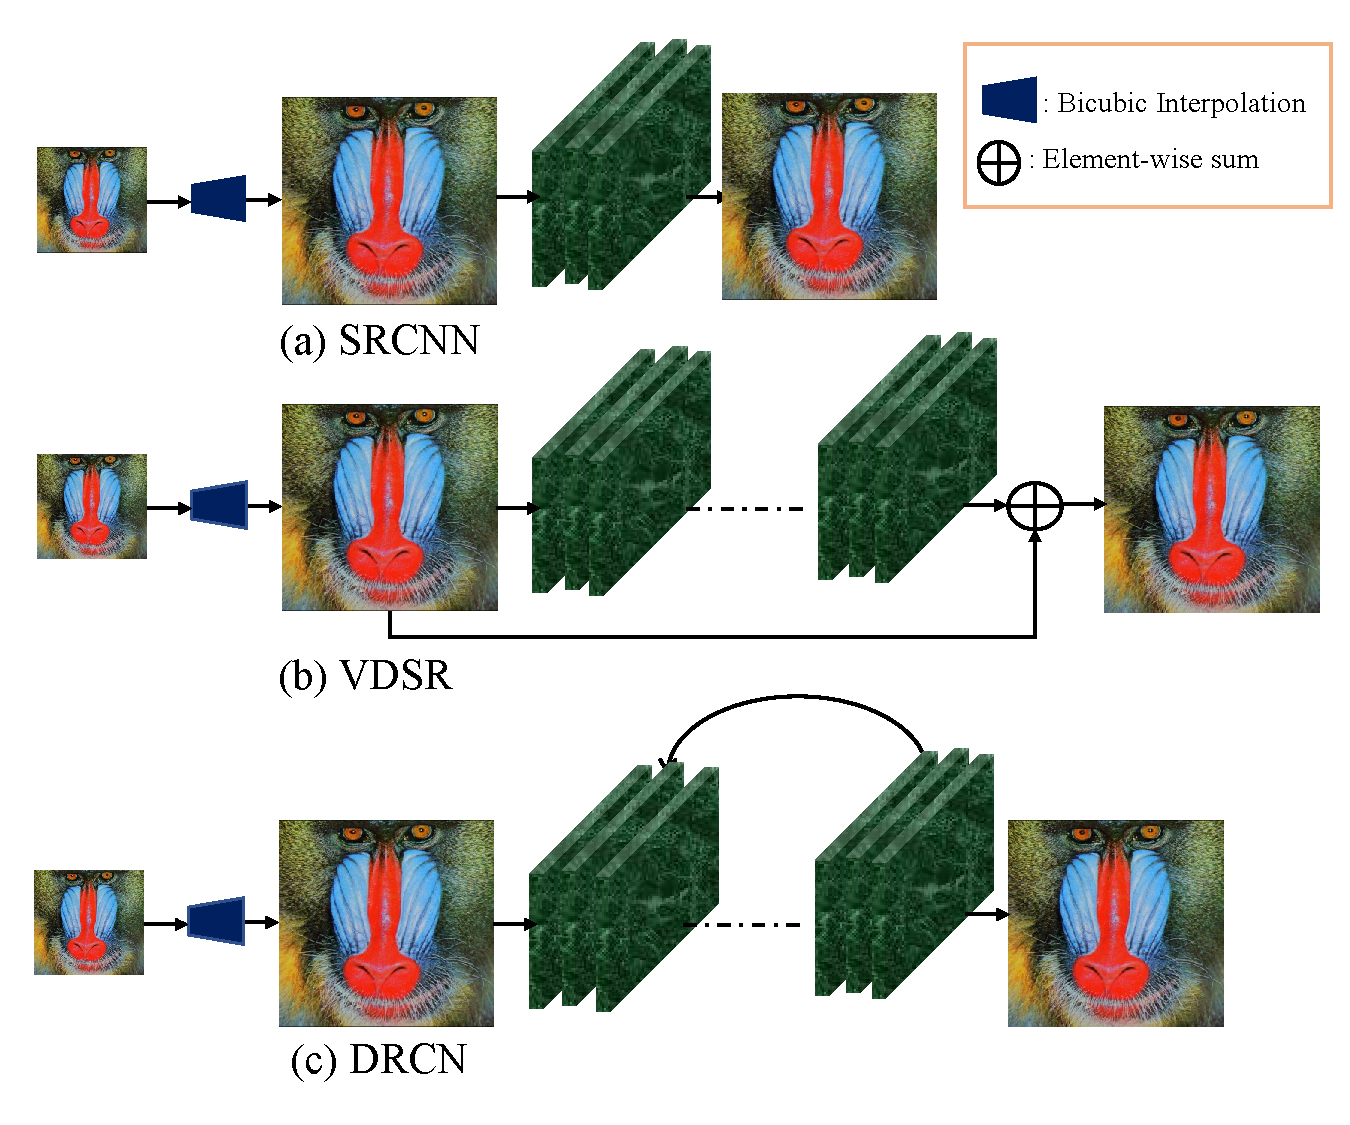
\includegraphics[width=\linewidth]{1FIGURE.pdf}}
    \caption {Pre-processing interpolation-based image super-resolution architectures of (a) SRCNN [6], (b) VDSR [9], and (c) DRCN [11].}

    \label{fig1}

\end{figure}




Furthermore, single local skip connection-based image super-resolution approaches face the loss of feature information at the subsequent end of the layers and act as a dead layer. This issue creates the vanishing gradient problem occurring in the training phase [8, 15, 16]. Our proposed model handles this issue with the support of global and local skip connections. In addition, selecting the proper activation function is crucial for developing deep CNN methods. Rectified linear unit (ReLU) activation function are currently the most popular activation function. As Krizhevsky \textit{et al.} [8], suggested that ReLU activation function performs a faster speed of the training and reduce the saturation problems. Still, several recent papers address the issues of exploding (i.e., retraining too much information) during the training [8, 15, 16]. It is desirable to suggest a novel activation function to address the abovementioned shortcomings. In contrast to ReLU and PReLU activation functions, the novel non-linear activation function proposed in this work is a LeakyReLU (LReLU) [15].
The main contribution of our proposed method is as under:

i) To reduce the computational cost and obtain the faster convergence during the training phase, we have replaced standard ResNet blocks with squeeze-and-excitation block (SEB) blocks which is inspired by the Squeeze and Excitation networks. Compared to other image SR methods, our suggested model outperformed them by a factor of $\times2$, $\times3$, $\times4$, and $\times8$ benchmark not only in speed but also in terms of computational cost.


ii) The deeper model faces the problems of Dying ReLU, which means the condition in which many ReLU neurons send output values as zero, and the whole network gets stuck and never improves the performance. We have replaced the ReLU with the LReLU activation function to initiate the dead features introduced by zero gradients.

iii) The single local and global skip connection does not reconstruct the visually pleasing high-quality HR image and introduces blurry artifacts to the HR output image. We have adopted a different approach and extracted the features information from the multi-local, sub-local, and global skip connections to reconstruct the visually pleasing, high-quality HR image.

The remaining sub-section of our work is explained as follows. Section II discusses the related work of deep CNN image SR methods. Section III explains the proposed method for SISR in detail. In section IV, we discussed the experimental  results with other state-of-the-art methods. Finally, section V explains the conclusions  and future work.


\section{RELATED WORK}
The objective of SISR is to reconstruct the visually appealing HR output image that contains detailed information from a LR input image. Conventional methods [1-5] was resolve the image SR problem differently, but deep learning-based CNN architecture used an effective and efficient way. In this section, we will mainly discuss the recent deep learning-based image SR approaches. The first deep learning-based solution to the SISR problem proposed by Dong \textit{et al.} [6] named as super-resolution convolutional neural network (SRCNN). SRCNN [6] model depends on three CNN layers to predict the output from the interpolated version of the upscaled image to reconstruct the HR image. Although, there is some weakness in this model. First, the proposed model used bicubic interpolation to upscale the original LR image, but bicubic interpolation introduced blurry results and did not design for this purpose. Second, image reconstruction information is still not satisfactory. The third is the slow convergence rate which takes more training time. Wang \textit{et al.} [17] introduce the sparse prior network for reconstructing the HR image, known as the Sparse Coding Network (SCN) [17]. The computational performance of SCN is also improved to earlier SR method [6]. Wang \textit{et al.} modified the model and replaced the non-linear mapping with a set of coding sparse sub-networks [18]. The main disadvantage of SCN [17] network architecture is the higher computational cost, leading to many problems in real-time applications.
To speed up the reconstruction process of image super-resolution, Dong \textit{et al.} introduced the  fast super-resolution CNN (FSRCNN) [7] architecture. FSRCNN [7] is an upgraded and faster version of the SRCNN [6] design. The straightforward network design of FSRCNN used one deconvolution layer and four CNN layers to upsample the original input LR images without using interpolation techniques. Compared to SRCNN  [7] performs better and has lower computational complexity, but still it has a smaller network capacity. Efficient sub-pixel convolutional neural network (ESPCN) [10] is a simple, efficient, and fast image super-resolution method, that can apply to real-time image and video applications.
A Very Deep Super-Resolution (VDSR) network with residual skip connection was introduced by  Kim \textit{et al.} [9] which was modeled after the visual geometry group network (VGGNet) used in the ImageNet for classification [8] task. VDSR employed the global residual learning connection with a faster convergence rate to lower the training complexity. The VDSR [9] method uses the bicubic interpolation-based upscaled input image rather than the actual pixel values resulting in increased memory usage and high computational costs. In addition, Kim  \textit{et al.} presented a Deeply Recursive Convolutional Network (DRCN) [11] for an image SR framework that employs several convolution layers. The key advantage of DRCN [11] is that it has constant training parameters (number of parameters). Although there are more recursions, the main drawback of DRCN [11] is that it slows the process of training convergence. The authors also applied the skip connection recursively to enhance model performance. The residual encoder-decoder networks (RED) are a notion that Mao \textit{et al.} extend and proposed the RED [19] model. In this approach authors used a residual learning with symmetric convolution operation to obtain the better performance. As a result, these findings support the idea that "the Deeper the Better." Contrarily, a shallow and deeper, fast deep learning-based approach was proposed by Romano \textit{et al.} named Rapid and Accurate Image Super-Resolution (RAISR) [20]. In this approach, the author classifies the input image patches concerning the angle of patches, coherence, and strength to learn the mappings from the original LR image to reconstruct the HR image. To rebuild the HR image, Lai  \textit{et al.} developed a deep Laplacian Pyramid Super-Resolution Network (LapSRN) [21], a novel image SR design. The LapSRN [21] architecture is based on many pyramid layers, each of which has a deconvolution layer acting as an upsample. Denoising convolutional neural networks (DnCNNs) were suggested by Zhang  \textit{et al.} [22] to speed up the development of an extremely deep convolutional neural network design.  The DnCNNs network stacks convolutional neural networks with Batch Normalization (BN) layer before the ReLU activation function, just like the SRCNN [6] network. Despite producing positive results, the model is computationally expensive because it uses a BN layer. Excessive use of convolution operations will limit the advancement of image super-resolution technology, especially for low-power computing devices. To resolve said issue, Zheng  \textit{et al.} [23] proposed the concept of a lightweight information multi-distillation network (IMDN). To further improve the performance of SR methods  Tai \textit{et al.} [24] developed a 52-layer Deep Recursive Residual Network called DRRN. Ledig  \textit{et al.} [25] use a deep CNN with residual skip connections having 16 blocks to recover the upsampled version of an output image. Lim \textit{et al.} [26] suggested an improved deep super-resolution network architecture to boost the model's training effectiveness and win the NTIRE 2017 SR Challenge [27] as well as produced the cutting-edge results named as enhanced deep super-resolution network (EDSR).  Tai \textit{et al.} proposed the deepest model for image restoration is a very deep persistent memory network (MemNet) and used several memory blocks to create persistent memory [28]. MemNet consists of cascaded memory blocks, which fuse the global features.

Yamanaka \textit{et al.} [29] developed a deep convolutional neural network-based framework for image SR to combine the parallel CNN layers with skip connections. The two networks they use most frequently are the SR image reconstruction network and a feature extraction network for extracting features from various levels. Compared to VDSR [9], this model is shallower. Han \textit{et al.} proposed a dual state recurrent networks (DSRN), which transmits information from the LR image state to the HR image state [30]. Authors update the signal information at each step before forwarding it to the HR state. A multi-scale residual network (MSRN) was created by Li \textit{et al.} [31]  and used the features fusion at various sizes by employing an adaptive feature detection strategy. This method utilized the full hierarchical-based feature type information to recreate the super-resolved HR image. Ahn  \textit{et al.} [32] suggested a method  for handling multi-scale information and learning residuals in LR feature space to select an appropriate paths [32]. Furthermore, this method [32] provides modules for scale-specific upsampling types with multiple shortcut connections. Choi  \textit{et al.} [33] used a recursive neural network and proposed a fast and efficient image SR with block state-based recursive network (BSRN). This type of network architecture tracks the current information status for image features. Zhang  \textit{et al.} [34] proposed the super-resolution network for multiple degradations (SRMD) to reconstructs the HR image by concatenating a LR image with its degradation mapping function. Furthermore, SRMD also designed another fine-tuning-based architecture named as noise-free degradation (SRMDNF) model [34] . Multi-scale inception-based super-resolution (SR) using deep learning (MSISRD) approach was proposed by Muhammad \textit{et al.} [35], to utilize the inception block to reconstruct the multi-scale feature information for image SR. In MSISRD approach author employed the concept of asymmetric convolution operation to reduce the model's computational cost. Wang  \textit{et al.} [36] demonstrated a dilated convolution neural network designed to expand the receptive field without expanding the kernel size. Furthermore, in [36] a shallow network architecture only increased the size of the receptive field. End-to-end image super-resolution via deep and shallow convolutional networks architecture provided short and long-range multi-scale information and replaced bicubic interpolation operation replaced with transposed CNN layer to reconstruct the HR image [37]. Yang  \textit{et al.} [38] proposed a transposed layer-based network architecture with large-scale components known as a deep recurrent fusion network (DRFN). Su \textit{et al.} [39] suggested a unique structure, which entails several sub-networks to reconstruct the HR image gradually and LR feature map used as an input for each sub-network. In image super-resolution, arbitrary enlargement factor is a challenge in real-time applications. Hui  \textit{et al.} [40] suggested an information distillation network (IDN) method to reconstruct the HR out image. In IDN [40] approach authors directly extract the features information from the original input LR image. IDN [40] uses a multiple cascaded information distillation block (DBlock) to reconstruct the residual-based high quality output image in HR domain. Hung \textit{et al.} [41] proposed a super-sampling network (SSNet) architecture to significantly reduces the number of parameters and multiplication operations due to the used of depthwise separable convolution operation. Barzegar \textit{et al.} [42] suggested a modest framework to avoid the training issue in the deeper network architecture. Multi-scale Xception Based Depthwise Separable Convolution for Single Image Super-resolution (MXDSIR) was proposed by Muhammad \textit{et al.} [43]. MXDSIR employed a depthwise separable convolution operation to reduce computational complexity. Hsu \textit{et al.} [44] were motivated by a capsule neural networks to extract additional possible feature information for image SR and created the two networks for image SR, such as the Capsule Image Restoration Neural Network (CIRNN) and the Capsule Attention and Reconstruction Neural Network (CARNN). For SR objectives and to learn the features information at various phases, Liu \textit{et al.} [45] presented a new hierarchical convolutional neural network (HCNN) architecture. The HCNN method involves a three-step hierarchical procedure based on the edge branch extraction, the edge reinforcement branch, and the SR image reconstruction branch. Prior knowledge and very sensitive to noise issued SR algorithm discussed in [46]. In this approach, the author fuses the information of multi-scale image information in a non-linear manner and uses a cascading-based multi-scale global mechanism to capture the non-local feature information. Xiao \textit{et al.} [47] introduced the idea of a powerful lightweight multi-scale feature extraction super-resolution network (MFEN) architecture. In the design of MFEN multi-scale feature extraction blocks (MFEBs) are stacked side-by-side to obtain multi-scale with hierarchical feature information. Xiao \textit{et al.} [47] also proposed a simple version of MFEN known as MFEN\texttt{\_}S.  To resolve the issues of network depth as well as width, Qin \textit{et al.} proposed an Attentive Residual Refinement Network (ARRFN) [48] method. Generally, the architecture of ARRFN consists of feature extraction, multi-scale separable upsampling blocks, and attentive residual refinement. Li \textit{et al.} proposed an adjustable SR network (ASRN) [49], which is easily adjusts the network depth of the proposed ASRN model.


\begin{figure*}
    \centering

    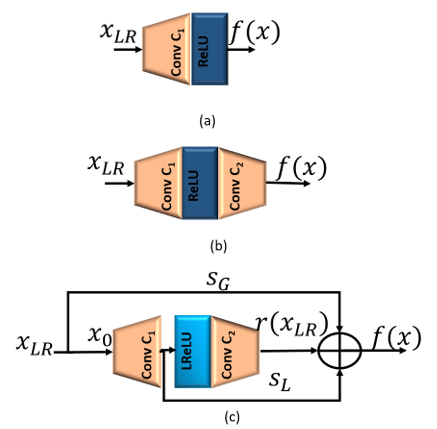
\includegraphics[width=\linewidth]{2Figure.pdf}
    \caption{The proposed framework of Squeeze-and-ExcitationNext for Single Image Super-Resolution (SENext).}
    \label{fig:2}
\end{figure*}

\section{PROPOSED METHOD}
In this section, we have discussed a detailed explanation of our proposed network architecture for SISR known as Squeeze-and-ExcitationNext for Single Image Super-Resolution (SENext), as shown in Figure 2.  The proposed framework mainly consists of two paths with four different types of blocks such as shallow feature extraction block (SFEB), squeeze-and-excitation block (SEB), split-concatenate block (SCB), and finally capsule unit block (CUB) with the support of special upper branch block (UBB). The information transfer pathway passes low, mid, and high-frequency information from the original low-resolution images.
In our proposed method, do not change the size of the input image. Initially, we extract the feature information from the original LR input image, add them, and pass through the SCB, followed by the CUB block. To reconstruct the visually pleasing HR output, we used all feature information with a special upper branch, and then the resultant output pass through the learning-based transposed convolution layer.




\begin{figure}[ht]
  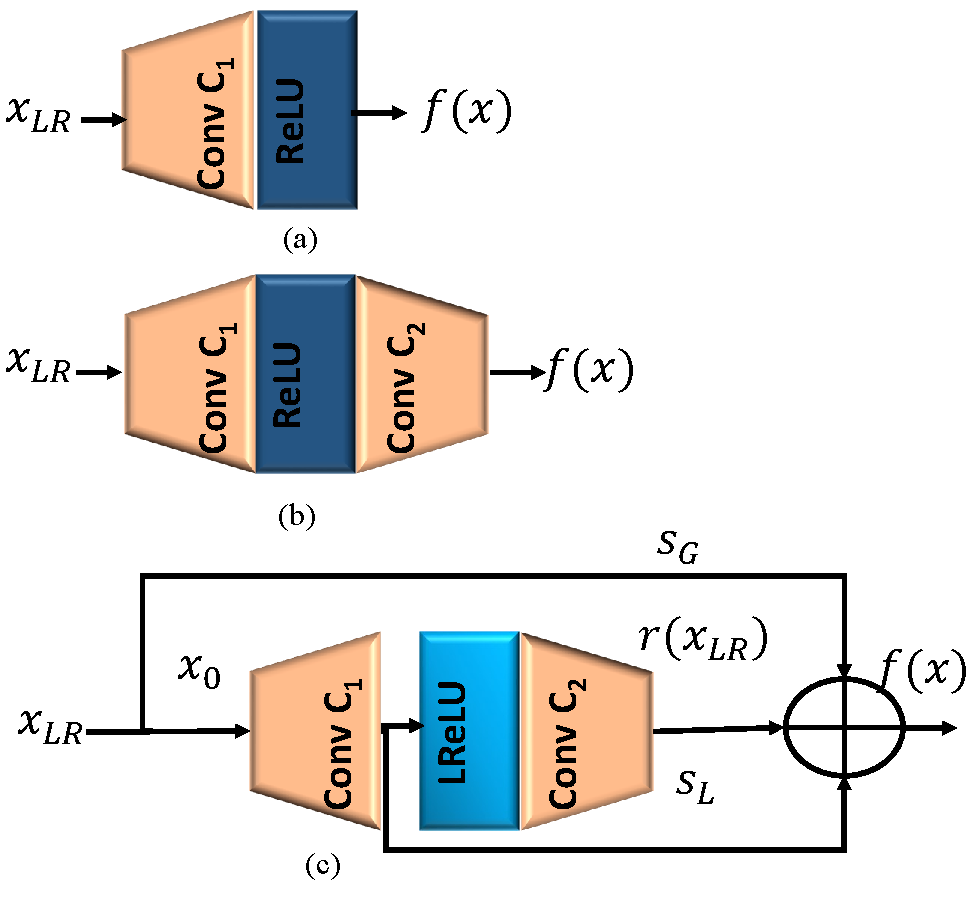
\includegraphics[width=\linewidth]{3FIGURE.pdf}
  \caption{Different types of Shallow feature extraction blocks are (a) Single layer shallow feature extraction block (b) Two-layer shallow feature extraction block, and (c) Our Proposed Shallow feature extraction block (SFEB).}
  \label{fig:7}
\end{figure}


\subsection{Shallow Feature Extraction Block (SFEB)}
According to the survey of [26, 50], the shallow feature $F_0$ is extracted from the original LR input image using only one or two $3\times3$ convolutional layers followed by the ReLU activation function, as shown in Figure 3(a) and 3(b). The design of said block is straightforward, but it cannot extract the complete shallow features information from the original LR input image. Furthermore, total network architecture depends on the initial shallow feature extractions, and sometimes essential feature information is lost when a network architecture is significantly deeper.   To extract the complete low and high-level features information from the original LR input image, we adapt the improved version of Figure 3(b) architecture with the use of local skip $S_L$ and global skip $S_G$ connections as shown in Figure 3(c). Our proposed, designed shallow feature extraction block is explained as:


\begin{equation}
{x_{0}}= {H_{SFEB}}({x_{LR}}\downarrow),
\end{equation}
where ${H_{SFEB}}$$(.)$ represents convolution operation, and $({x_{LR}}\downarrow)$ is the original input LR image. After obtaining the shallow features ${x_{0}}$ is then used as the input of SEB.
\subsection{ squeeze-and-excitation block (SEB)}
For image and computer vision-based applications, the SqueezeNet deep CNN architecture mainly focuses on computational cost and model efficiency [51]. The first basic architecture of the SqueezeNet block is commonly known as a fire module, as shown in Figure 4. The whole architecture consists of two stages: a squeeze stage that applies a series of $1\times1$ kernel and the expanded stage use $3\times3$ kernels both followed by a conventional ReLU) activation function. The number of squeeze filters that can be learned is always less than the volume of the input. Consequently, the squeeze stage may be considered a dimensionality reduction process that also captures the pixel correlations between input channels. The output of the squeezing phase relates to the expansion phase, which combines learning $1\times1$ and $3\times3$ convolutions. To reduce the vanishing gradient issue during the training as well as decrease the computational complexity, we proposed an improved squeeze-and-excitation block (SEB) by stacking a series of $1\times1$ convolution layers in each phase and using the LReLU activation function in place of the ReLU activation function as shown in Figure 5. Suppose the proposed SEB contains N number of Blocks, then $x_{n-1}$ and $x_n$ be the input and output of the $n^{th}$ SEB block. The resultant output of $x_n$ feed to the SCB block.

\begin{figure*}
    \centering

    \includegraphics[width=\linewidth]{4Figure.pdf}
    \caption{Original Fire Block (Squeeze and Expand Stage Block).}
    \label{fig:4}
\end{figure*}

\begin{figure*}
    \centering

    \includegraphics[width=\linewidth]{5Figure.pdf}
    \caption{Proposed fire module used as a squeeze and excitation (SEB) block .}
    \label{fig:5}
\end{figure*}


\begin{equation}
{x_{n}}= {H_{n}}({x_{n-1}}), = {H_{n}}({x_{n-1}})(...({H_{1}}({x_{0}}))...),
\end{equation}
\subsection{Split-concatenation block (SCB)}
Residual learning is one of the most crucial technique to ease the training for large-scale networks [52]. A global skip connection was implemented by Kim \textit{et al.} in [9] and could concentrate on predicting the residual skip connection learning. Furthermore, residual skip connection technique moved the extracted feature information through every block using the short-term skip connections [53]. Numerous efforts have altered the structure of original ResNet [52] was first time developed for the image recognition task and obtained the remarkable performance. Several versions of the residual learning-based construction blocks are shown in Figures 6(a) and 6(b). The SRResNet building block [25]  differs from the original ResNet block [52], due to the lacking of an activation layer following element-wise addition. The two BN layers were eliminated from SRResNet to create the EDSR building blocks [26]. The authors of EDSR [26] are recommended that BN would not be appropriate for the image super-resolution task. Thus, our proposed model adopts a split-concatenate block without BN, as shown in Figure 6(c). Initially, HR features are split into two branches with a kernel size of $3\times3$ and $5\times5$ to take the benefit of small as well as a sizeable receptive field both followed by another $3\times3$ filter with LReLU activation function to prevents gradients from saturating and mitigates the risk of vanishing gradients.

\begin{figure}[ht]
  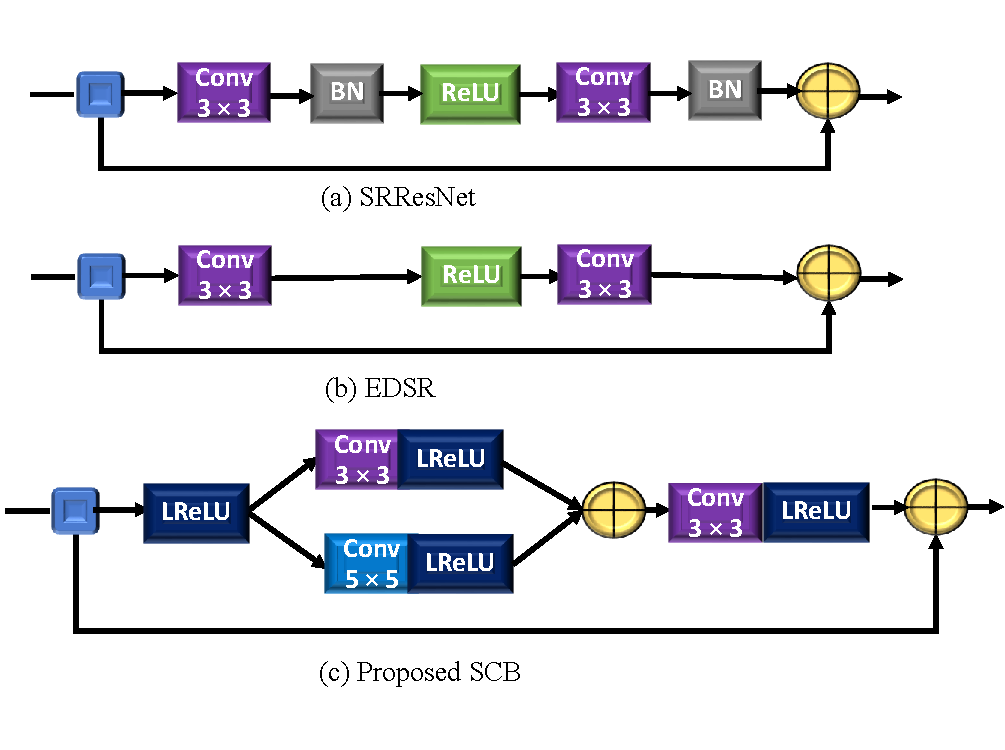
\includegraphics[width=\linewidth]{6FIGURE.pdf}
  \caption{The structures of different residual learning blocks. (a) SRResNet [25], (b) EDSR [26], and (c) Our proposed Split-Concatenate Block (SCB).}
  \label{fig:7}
\end{figure}



\subsection{capsule unit block (CUB)}
To minimize the feature map dimension and merge long-term features with skip connections to rebuild the high-quality HR image, a Squeeze Unit is introduced [54]. To follow the concept of [54], we proposed a particular capsule unit block (CUB) with a global skip connection, as shown in Figure 7. The design of the proposed CUB block consists of one bottleneck layer followed by LReLU and one $3\times3$ filter. The bottleneck layer recalibrates the information with a sub-local skip connection to overcome parameter growth and build an efficient architecture. The concatenated output is used by one convolution layer of filter size is $3\times3$.


\begin{figure}[ht]
  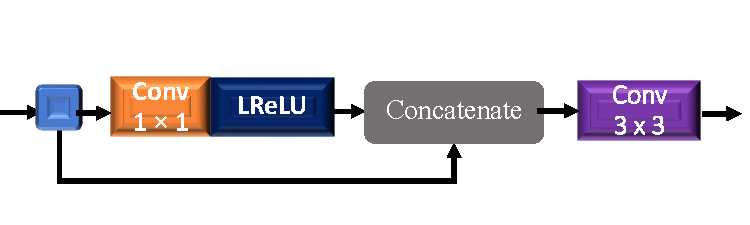
\includegraphics[width=\linewidth]{7FIGURE.pdf}
  \caption{Proposed Capsule Unit Block (CUB) with local skip connection.}
  \label{fig:7}
\end{figure}



\subsection{Upper branch block (UBB)}
Implementation of Inception [55] network architecture-based block before the transpose layer to extract the multi-scale features information is to increase the computational cost. Furthermore, inception block used before the transposed layer is to availability of a max-pooling layer. The max-pooling layer is to lose the features information, which leads to drop the performance of the model [56, 57]. Furthermore, $5\times5$ kernel size is more time-consuming and expensive. To resolve these issues, we proposed an alternate design with a simple upper branch block (UBB) with a small kernel size as shown in Figure 8. We removed the max-pooling layer operation with a residual skip connection. In the UBB block, we utilized $10$ CNN layers having a filter size is $3\times3$ with the support of the LReLU function, except the last layer. The resultant LR features are concatenated and fed through the learning-based deconvolution layer with a filter size is $3\times 3$ to recover the visually pleasing HR reconstructed output image.

\begin{figure}[ht]
  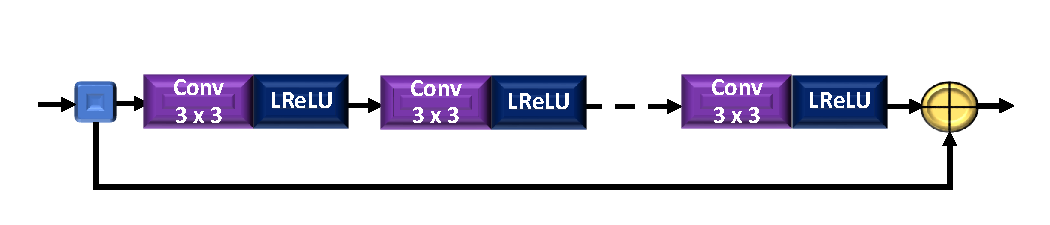
\includegraphics[width=\linewidth]{8FIGURE.pdf}
  \caption{Proposed Upper Branch Block (UBB) with global skip connection.}
  \label{fig:8}
\end{figure}



\section{Experimental Results}
In this section, we assess the effectiveness of our SENext model on different public datasets. Initially, we discuss the training and testing datasets; then, we will explain the experimental evaluations with state-of-the-art methods. Training was performed on a combination of two datasets, such as 100 image of DIV2K [27] and 300 images of BSDS300 [58].  The same combination is observed in [50, 59]. Additionally, we apply the data augmentation technique to decrease the chances of overfitting and increase the efficiency during the training. For experimental calculations we used the five benchmark test datasets, such as Set5 [60] , Set14 [61] , BSDS100 [58], Urban100  [62]  and Manga109  [63]. The original low-resolution image is obtained using MATLAB bicubic operation for enlargement scale factor $\times 2$, $\times 3$, $\times 4$, and $\times 8$. Adam optimizer used for training purposes with 0.0001 initial learning rate. The proposed methods used the Windows 11 operating system having one GPU (GeForce NVIDIA RTX 2070 GPU) with  Core (TM) i7-9750H CPU of an Intel(R) @ 2.60GHz having 16.0 GB RAM system. The training and testing phase is performed under Keras 2.6.0 with TensorFlow 2.6.0 environment.
\subsection{Quantitative comparisons with existing state-of-the-art-methods}
The quantitative comparison analysis of five benchmark test datasets is present in a Table 1. Our proposed SENext quantitatively compare with fourteen methods, such as Bicubic, SRCNN [6], FSRCNN [7], VDSR [9], DRCN [11], LapSRN [21], DRRN [24], MemNet [28], ASRN [49], IDN [40], SRMDNF [34], MFEN\texttt{\_}S [47], CARN [32], and IMDN [40]. 
As seen in Table 1, our SENext quantitative (PSNR/SSIM) results are significantly outperformed as compare to state-of-the-art methods. Performance of SENext model is better on almost test datasets except Set5 scale factor $3\times$ and $4\times$. Furthermore, on all over average our model obtained higher value of PSNR/SSIM than other methods.

\begin{figure}[ht]
  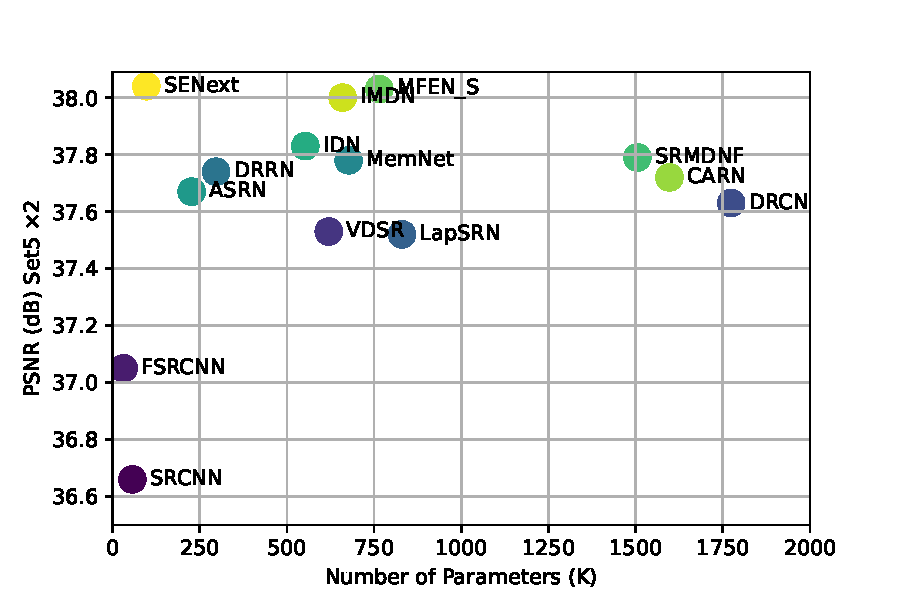
\includegraphics[width=\linewidth]{9FIGURE.pdf}
  \caption{The performance comparison in terms of model parameters versus PSNR tested on the image dataset of Set5 with upscale factor $\times2$.}
  \label{fig:10}
\end{figure}





\begin{table*}
\caption{Presents the quantitative assessment of image SR methods with our SENext. The reported results of average values of PSNR/SSIM of factors $\times 2$, $\times 3$ $\times 4$, and $\times 8$. {\color{red}\textbf{Red }} color with bold quantitative values is recorded as the best value. The {\color{blue}\underline{blue}} color with underlined quantitative values is indicated as the 2nd best value.}

\label{table1}
\setlength{\tabcolsep}{4.5 pt}
\begin{tabular}{|c|c|c|cc|cc|cc|cc|cc|cc|}
\hline
\multirow{2}{*}{Method} & \multirow{2}{*}{Factor} & \multirow{2}{*}{Para}& \multicolumn{2}{c|}{Set5}& \multicolumn{2}{c|}{Set14}& \multicolumn{2}{c|}{BSDS100}& \multicolumn{2}{c|}{Urban100}& \multicolumn{2}{c|}{Manga109}& \multicolumn{2}{c|}{Average}\\


 \cline{4-15}&&& \multicolumn{1}{c|}{PSNR$\uparrow$}  & SSIM{$\uparrow$}   & \multicolumn{1}{c|}{PSNR$\uparrow$}  & SSIM {$\uparrow$}   & \multicolumn{1}{c|}{PSNR$\uparrow$}  & SSIM {$\uparrow$}   & \multicolumn{1}{c|}{PSNR$\uparrow$}  & SSIM {$\uparrow$}  & \multicolumn{1}{c|}{PSNR$\uparrow$}  & SSIM {$\uparrow$}   & \multicolumn{1}{c|}{PSNR$\uparrow$}  & SSIM {$\uparrow$}  \\
 \hline

Bicubic&$\times2$ & -/-& \multicolumn{1}{c|}{33.66 } & 0.9299  & \multicolumn{1}{c|}{30.24 } &0.8688  & \multicolumn{1}{c|}{29.56 } & 0.8431  & \multicolumn{1}{c|}{26.88 } & 0.8403  & \multicolumn{1}{c|}{30.80 } & 0.9339&
\multicolumn{1}{c|}{30.23} & 0.8832 \\


SRCNN[6] & $\times 2$ & 57K& \multicolumn{1}{c|}{36.66 } & 0.9542  & \multicolumn{1}{c|}{32.45 } & 0.9067  &\multicolumn{1}{c|}{31.36 } & 0.8879  & \multicolumn{1}{c|}{29.50 } &0.8946 & \multicolumn{1}{c|}{35.60} &0.9663
&\multicolumn{1}{c|}{33.11} & 0.9219\\

FSRCNN[7]& $\times 2$& 12K & \multicolumn{1}{c|}{37.05} &0.9560& \multicolumn{1}{c|}{32.66} & 0.9090 &\multicolumn{1}{c|}{31.53} &0.8920& \multicolumn{1}{c|}{29.88} &0.9020& \multicolumn{1}{c|}{36.67} &0.9710
&\multicolumn{1}{c|}{33.56} & 0.9260\\


VDSR[9]& $\times 2$&665K& \multicolumn{1}{c|}{37.53} & 0.9590 & \multicolumn{1}{c|}{33.05} & 0.9130 &\multicolumn{1}{c|}{31.90} & 0.8960& \multicolumn{1}{c|}{30.77} & 0.9140 & \multicolumn{1}{c|}{37.22} & 0.9750
&\multicolumn{1}{c|}{33.24} & 0.9314\\



DRCN[11]& $\times 2$&1,774K& \multicolumn{1}{c|}{37.63} & 0.9588 & \multicolumn{1}{c|}{33.04} &0.9124 &\multicolumn{1}{c|}{31.85} & 0.8942& \multicolumn{1}{c|}{30.75} &0.9133 & \multicolumn{1}{c|}{37.55} & 0.9732
&\multicolumn{1}{c|}{34.16} & 0.9304\\


LapSRN[21] & $\times 2$&813K& \multicolumn{1}{c|}{37.52} & 0.9590 & \multicolumn{1}{c|}{33.08} & 0.9130 &\multicolumn{1}{c|}{31.08} & 0.8950 & \multicolumn{1}{c|}{30.41} &  0.9101 & \multicolumn{1}{c|}{37.27} &  0.9740
&\multicolumn{1}{c|}{33.87} & 0.9302\\

DRRN[24]& $\times 2$&297K& \multicolumn{1}{c|}{37.74} &  0.9591  & \multicolumn{1}{c|}{33.23 } & 0.9136  &\multicolumn{1}{c|}{32.05} & 0.8973 & \multicolumn{1}{c|}{31.23} & 0.9188 & \multicolumn{1}{c|}{37.60} & 0.9736
&\multicolumn{1}{c|}{34.37} &0.9325\\


MemNet [28] & $\times 2$&677K& \multicolumn{1}{c|}{37.78} & 0.9597  & \multicolumn{1}{c|}{33.28} &0.9142  &\multicolumn{1}{c|}{32.08} & 0.8978 & \multicolumn{1}{c|}{31.31} &0.9195  & \multicolumn{1}{c|}{37.72} &0.9740
&\multicolumn{1}{c|}{34.43} &0.9330\\


ASRN [49]& $\times 2$&227K& \multicolumn{1}{c|}{37.67} &0.9594 & \multicolumn{1}{c|}{33.19} & 0.9144 &\multicolumn{1}{c|}{31.95} &0.8970& \multicolumn{1}{c|}{31.20} &0.9186 & \multicolumn{1}{c|}{37.79} & 0.9753
&\multicolumn{1}{c|}{34.36} &0.9329\\

IDN [40] & $\times 2$&553K& \multicolumn{1}{c|}{37.83} & 0.9600 & \multicolumn{1}{c|}{33.30} & 0.9148  &\multicolumn{1}{c|}{32.08} & 0.8985 & \multicolumn{1}{c|}{31.27} & 0.9196  & \multicolumn{1}{c|}{38.01} & 0.9749
&\multicolumn{1}{c|}{34.50} &0.9336\\


SRMDNF [34] & $\times 2$&1,511K& \multicolumn{1}{c|}{37.79} & 0.9601  & \multicolumn{1}{c|}{33.32} & 0.9159  &\multicolumn{1}{c|}{32.05} & 0.8985 & \multicolumn{1}{c|}{31.33} &0.9204& \multicolumn{1}{c|}{38.07} & 0.9761
&\multicolumn{1}{c|}{34.51} &0.9342\\


MFEN\texttt{\_}S [47] & $\times 2$&755K& \multicolumn{1}{c|}{\color{blue}\underline{38.03}} & {\color{blue}\underline{0.9606}} & \multicolumn{1}{c|}{33.55} & 0.9171  &\multicolumn{1}{c|}{\color{blue}\underline{32.19}} &{\color{red}\textbf{0.9283}} & \multicolumn{1}{c|}{\color{blue}\underline{32.19}} & 0.8997 & \multicolumn{1}{c|}{38.77} &0.9772
&\multicolumn{1}{c|}{34.95} & {\color{blue}\underline{0.9366}}\\


CARN [32] & $\times 2$ &1,592K& \multicolumn{1}{c|}{37.76} & 0.9590 & \multicolumn{1}{c|}{33.52} & 0.9166 & \multicolumn{1}{c|}{32.09} & 0.8978 & \multicolumn{1}{c|}{31.92} &0.9266 & \multicolumn{1}{c|}{38.36} & 0.9765
&\multicolumn{1}{c|}{34.73} & 0.9353\\


IMDN [40] & $\times 2$ &694K& \multicolumn{1}{c|}{38.00} & 0.9605 & \multicolumn{1}{c|}{\color{blue}\underline{33.63}} &{\color{blue}\underline{ 0.9177}} & \multicolumn{1}{c|}{\color{blue}\underline{32.19}} & 0.8996& \multicolumn{1}{c|}{32.17} & {\color{blue}\underline{0.9283}} & \multicolumn{1}{c|}{\color{red}\textbf{38.88}} &{\color{red}\textbf{0.9784}}
&\multicolumn{1}{c|}{\color{blue}\underline{34.97}} &  0.9369\\


SENext (Our) & $\times 2$ &97K& \multicolumn{1}{c|}{\color{red}\textbf{38.04}} &{\color{red}\textbf{0.9608}} & \multicolumn{1}{c|}{\color{red}\textbf{34.24} } &{\color{red}\textbf{ 0.9181}} & \multicolumn{1}{c|}{\color{red}\textbf{32.21}} &{\color{blue}\underline{0.8997}}& \multicolumn{1}{c|}{\color{red}\textbf{32.43}} &{\color{red}\textbf{0.9287}}& \multicolumn{1}{c|}{\color{blue}\underline{38.79}} &{\color{blue}\underline{0.9774}} &\multicolumn{1}{c|}{\color{red}\textbf{35.14}} & {\color{red}\textbf{0.9369}}\\
\hline

Bicubic&$\times3$ &-/-& \multicolumn{1}{c|}{30.39} & 0.8682  & \multicolumn{1}{c|}{27.55} & 0.7742 & \multicolumn{1}{c|}{27.21} & 0.7385 & \multicolumn{1}{c|}{24.46} & 0.7349  & \multicolumn{1}{c|}{26.95} &0.8566
&\multicolumn{1}{c|}{27.31} & 0.7945\\

SRCNN[6] & $\times3$ & 57K&\multicolumn{1}{c|}{32.75} & 0.9090  & \multicolumn{1}{c|}{29.30} & 0.8215  &\multicolumn{1}{c|}{28.41} & 0.7863  & \multicolumn{1}{c|}{26.24} &0.7989 & \multicolumn{1}{c|}{30.48} &0.9117
&\multicolumn{1}{c|}{29.44} & 0.8455\\


FSRCNN[7]& $\times3$ &12K& \multicolumn{1}{c|}{33.18} &0.9140& \multicolumn{1}{c|}{29.37} & 0.8240 &\multicolumn{1}{c|}{28.53} & 0.7910& \multicolumn{1}{c|}{26.34} &0.8080& \multicolumn{1}{c|}{31.10} &0.9210
&\multicolumn{1}{c|}{29.70} & 0.8516\\

VDSR[9]& $\times3$ &665K& \multicolumn{1}{c|}{33.66} & 0.9213 & \multicolumn{1}{c|}{29.77} & 0.8314 &\multicolumn{1}{c|}{28.82} & 0.7976& \multicolumn{1}{c|}{27.14} & 0.8279 & \multicolumn{1}{c|}{32.01} & 0.9340
&\multicolumn{1}{c|}{30.28} & 0.8624\\



DRCN[11]&$\times3$ &1,774K& \multicolumn{1}{c|}{33.82} & 0.9226 & \multicolumn{1}{c|}{29.76} &0.8311 &\multicolumn{1}{c|}{28.80} & 0.7963& \multicolumn{1}{c|}{27.15} &0.8276 & \multicolumn{1}{c|}{32.24} & 0.9343
&\multicolumn{1}{c|}{30.35} & 0.8624\\

LapSRN[21] &$\times3$ &813K& \multicolumn{1}{c|}{33.82} & 0.9227  & \multicolumn{1}{c|}{29.87} & 0.8320  &\multicolumn{1}{c|}{28.82} & 0.7980  & \multicolumn{1}{c|}{27.07} & 0.8280 & \multicolumn{1}{c|}{32.21} & 0.9350
&\multicolumn{1}{c|}{30.36} & 0.8631\\



DRRN[24]& $\times3$ &297K& \multicolumn{1}{c|}{34.03} &  0.9244 & \multicolumn{1}{c|}{29.96} & 0.8349 &\multicolumn{1}{c|}{28.95} & 0.8004 & \multicolumn{1}{c|}{27.53} & 0.8378 & \multicolumn{1}{c|}{32.71} & 0.9379
&\multicolumn{1}{c|}{30.64} &  0.8671\\

MemNet [28] & $\times3$ &677K& \multicolumn{1}{c|}{34.09} &0.9248  & \multicolumn{1}{c|}{30.00} &0.8350  &\multicolumn{1}{c|}{28.96} & 0.8001 & \multicolumn{1}{c|}{27.56} & 0.8376 & \multicolumn{1}{c|}{32.51} &0.9369
&\multicolumn{1}{c|}{ 30.62} &0.8669\\


ASRN [49]& $\times3$&248K& \multicolumn{1}{c|}{33.84} & 0.9223 & \multicolumn{1}{c|}{29.97} & 0.8348 &\multicolumn{1}{c|}{28.86} & 0.7990& \multicolumn{1}{c|}{27.41} & 0.8342 & \multicolumn{1}{c|}{32.63} & 0.9364
&\multicolumn{1}{c|}{30.54} &0.8653\\


IDN [40] & $\times3$&553K& \multicolumn{1}{c|}{34.11} & 0.9253 & \multicolumn{1}{c|}{29.99} & 0.8354 &\multicolumn{1}{c|}{28.95} & 0.8013 & \multicolumn{1}{c|}{27.42} & 0.8359 & \multicolumn{1}{c|}{32.71} & 0.9381
&\multicolumn{1}{c|}{30.64} &0.8672\\



SRMDNF [34] & $\times3$ &1,528K& \multicolumn{1}{c|}{34.12} & 0.9254& \multicolumn{1}{c|}{30.04} &0.8382 &\multicolumn{1}{c|}{28.97} & 0.8025& \multicolumn{1}{c|}{27.57} & 0.8398& \multicolumn{1}{c|}{33.00} & 0.9403
&\multicolumn{1}{c|}{30.74} &0.8692\\



CARN [32] & $\times3$ &1,592K& \multicolumn{1}{c|}{34.29} &{\color{blue}\underline{0.9255}} & \multicolumn{1}{c|}{30.29} & 0.8407 & \multicolumn{1}{c|}{29.06} & 0.8034 & \multicolumn{1}{c|}{28.06} & {\color{blue}\underline{0.8493}} & \multicolumn{1}{c|}{33.50} & 0.9440
&\multicolumn{1}{c|}{31.04} &0.8726\\



IMDN [40] & $\times3$ &703K& \multicolumn{1}{c|}{\color{red}\textbf{34.36}} & {\color{red}\textbf{0.9270}} & \multicolumn{1}{c|}{\color{blue}\underline{30.32}} &{\color{blue}\underline{0.8417}} & \multicolumn{1}{c|}{\color{blue}\underline{29.09}} & {\color{blue}\underline{0.8046}} & \multicolumn{1}{c|}{\color{blue}\underline{28.17}} & {\color{red}\textbf{0.8519}}& \multicolumn{1}{c|}{\color{blue}\underline{33.61}} &{\color{blue}\underline{0.9446}} &\multicolumn{1}{c|}{\color{blue}\underline{31.11}} & {\color{red}\textbf{0.8740}}\\


SENext (Our) & $\times3$ &54K& \multicolumn{1}{c|}{\color{blue}\underline{34.32}} &{\color{blue}\underline{0.9255}}& \multicolumn{1}{c|}{\color{red}\textbf{31.08}} & {\color{red}\textbf{0.8419}}& \multicolumn{1}{c|}{\color{red}\textbf{29.11}} &{\color{red}\textbf{0.8047}}& \multicolumn{1}{c|}{\color{red}\textbf{28.60}} &{\color{red}\textbf{0.8519}}& \multicolumn{1}{c|}{\color{red}\textbf{33.63}} &{\color{red}\textbf{0.9451}} &\multicolumn{1}{c|}{\color{red}\textbf{31.35}} &{\color{blue}\underline{0.8738}}\\

\hline

Bicubic&$\times4$ &-/-& \multicolumn{1}{c|}{28.42 } &0.8104 & \multicolumn{1}{c|}{26.00  } &0.7027& \multicolumn{1}{c|}{25.96 } & 0.6675  & \multicolumn{1}{c|}{23.14 } & 0.6577  & \multicolumn{1}{c|}{24.89} &0.7866

&\multicolumn{1}{c|}{25.68} &0.7250\\


SRCNN[6] & $\times4$  &57K& \multicolumn{1}{c|}{30.48 } &0.8628   & \multicolumn{1}{c|}{27.50 } &0.7513  &\multicolumn{1}{c|}{ 26.90 } & 0.7010 & \multicolumn{1}{c|}{24.52 } &0.7221 & \multicolumn{1}{c|}{27.58 } &0.8555
&\multicolumn{1}{c|}{ 27.40} &0.7785 \\


FSRCNN[7]& $\times4$ &12K& \multicolumn{1}{c|}{30.72} & 0.8660& \multicolumn{1}{c|}{27.61} &0.7550  &\multicolumn{1}{c|}{26.98} &0.7150 & \multicolumn{1}{c|}{24.62} &0.7280 & \multicolumn{1}{c|}{27.90 } &0.8610
&\multicolumn{1}{c|}{27.57} &0.7850 \\


VDSR[9]& $\times4$ &665K & \multicolumn{1}{c|}{31.35} &0.8838 & \multicolumn{1}{c|}{28.01} & 0.7674&\multicolumn{1}{c|}{27.29} &0.7251 & \multicolumn{1}{c|}{25.18} &0.7524 & \multicolumn{1}{c|}{28.83 } & 0.8870
&\multicolumn{1}{c|}{28.13} &0.8031 \\



DRCN[11]& $\times4$ &1,774K& \multicolumn{1}{c|}{31.53} &0.8854  & \multicolumn{1}{c|}{28.02 } &0.7670 &\multicolumn{1}{c|}{27.23} &0.7233 & \multicolumn{1}{c|}{25.14 } &0.7510 & \multicolumn{1}{c|}{28.93 } & 0.8854
&\multicolumn{1}{c|}{28.17 } &0.8024 \\


LapSRN [21] & $\times4$ &813K& \multicolumn{1}{c|}{31.54} &0.8850 & \multicolumn{1}{c|}{28.19} &0.7720  &\multicolumn{1}{c|}{27.32} &0.7270  & \multicolumn{1}{c|}{25.21 } &0.7560   & \multicolumn{1}{c|}{29.09 } &0.8900
&\multicolumn{1}{c|}{28.27 } &0.8060 \\


DRRN[24]& $\times4$ &297K& \multicolumn{1}{c|}{31.68} &0.8888 & \multicolumn{1}{c|}{28.21} &0.7720 &\multicolumn{1}{c|}{27.38} &0.7284 & \multicolumn{1}{c|}{25.44} &0.7638 & \multicolumn{1}{c|}{29.45} & 0.8946
&\multicolumn{1}{c|}{28.43} &0.8095  \\


MemNet [28] & $\times4$ &677K& \multicolumn{1}{c|}{31.74} &0.8893& \multicolumn{1}{c|}{28.26} &0.7723 &\multicolumn{1}{c|}{27.40} &0.7281& \multicolumn{1}{c|}{25.50} &0.7630& \multicolumn{1}{c|}{29.42} & 0.8942
&\multicolumn{1}{c|}{28.46} &0.8094\\


ASRN [49]& $\times4$ &244K& \multicolumn{1}{c|}{31.65} &0.8867 & \multicolumn{1}{c|}{28.28} & 0.7733 &\multicolumn{1}{c|}{27.34} &0.7279 & \multicolumn{1}{c|}{25.42} &0.7616 & \multicolumn{1}{c|}{29.59} & 0.8935
&\multicolumn{1}{c|}{28.46} &0.8086 \\


IDN [40] & $\times4$ &553K& \multicolumn{1}{c|}{31.82} &0.8903& \multicolumn{1}{c|}{28.25} &0.7730 &\multicolumn{1}{c|}{27.41} &0.7297 & \multicolumn{1}{c|}{25.41 } & 0.7632 & \multicolumn{1}{c|}{29.41} & 0.8942
&\multicolumn{1}{c|}{28.46} &0.8101  \\


SRMDNF [34] & $\times4$ &1,552K& \multicolumn{1}{c|}{31.96 } &0.8925 & \multicolumn{1}{c|}{28.35} &0.7787 &\multicolumn{1}{c|}{27.49} &0.7337& \multicolumn{1}{c|}{25.68} &0.7731 & \multicolumn{1}{c|}{30.09} &0.9024
&\multicolumn{1}{c|}{	28.71} &0.8161 \\

MFEN\texttt{\_}S [47] & $\times4$ &775K& \multicolumn{1}{c|}{32.23} &0.8951& \multicolumn{1}{c|}{28.61} &0.7814 &\multicolumn{1}{c|}{26.07} &0.7847& \multicolumn{1}{c|}{27.56} &0.7355& \multicolumn{1}{c|}{30.41} &0.9074
&\multicolumn{1}{c|}{\color{blue}\underline{28.98}} &{\color{red}\textbf{0.8208}} \\

CARN [32] & $\times4$  & 1,592K&\multicolumn{1}{c|}{\color{blue}\underline{32.13}} &{\color{blue}\underline{0.8937}} & \multicolumn{1}{c|}{\color{blue}\underline{28.60}} &0.7806& \multicolumn{1}{c|}{\color{blue}\underline{27.58}} &0.7349& \multicolumn{1}{c|}{\color{blue}\underline{26.07}} &0.7837& \multicolumn{1}{c|}{\color{blue}\underline{30.47}} &{\color{red}\textbf{0.9084}} &\multicolumn{1}{c|}{28.97} &0.8203 \\

IMDN [40] & $\times4$  &715K& \multicolumn{1}{c|}{\color{red}\textbf{32.21}} &{\color{red}\textbf{0.8948}} & \multicolumn{1}{c|}{28.58} &{\color{blue}\underline{0.7811}}& \multicolumn{1}{c|}{27.56} &{\color{blue}\underline{0.7353}} & \multicolumn{1}{c|}{26.04} &{\color{blue}\underline{0.7838}}& \multicolumn{1}{c|}{30.45} &{\color{blue}\underline{0.9075}} &\multicolumn{1}{c|}{28.97} &{\color{blue}\underline{0.8205}}  \\

SENext (Our) & $\times4$  &54K& \multicolumn{1}{c|}{31.50} &0.8947  & \multicolumn{1}{c|}{\color{red}\textbf{28.99}} &{\color{red}\textbf{0.7812}}  & \multicolumn{1}{c|}{\color{red}\textbf{28.49}} &{\color{red}\textbf{0.7357}} & \multicolumn{1}{c|}{\color{red}\textbf{26.64 }} &{\color{red}\textbf{0.7839}}  & \multicolumn{1}{c|}{\color{red}\textbf{30.48}} &{\color{red}\textbf{0.9084}}
&\multicolumn{1}{c|}{\color{red}\textbf{29.22}} &{\color{red}\textbf{0.8208}}    \\
\hline

Bicubic&$\times8$ &-/-& \multicolumn{1}{c|}{24.40} &0.6580& \multicolumn{1}{c|}{23.10} &0.5660 & \multicolumn{1}{c|}{23.67} &0.5480& \multicolumn{1}{c|}{20.74} &0.5160 & \multicolumn{1}{c|}{21.47} & 0.6500
&\multicolumn{1}{c|}{22.68} & 0.5876     \\


SRCNN[6] & $\times8$ &57K& \multicolumn{1}{c|}{25.34} & 0.6471 & \multicolumn{1}{c|}{23.86} &0.5443 &\multicolumn{1}{c|}{24.14} &0.5043 & \multicolumn{1}{c|}{21.29} &0.5133& \multicolumn{1}{c|}{22.46} &0.6606
&\multicolumn{1}{c|}{23.42} & 0.5739      \\

FSRCNN[7]& $\times8$&12K& \multicolumn{1}{c|}{25.42} &0.6440 & \multicolumn{1}{c|}{23.94} &0.5482&\multicolumn{1}{c|}{24.21} &0.5112 & \multicolumn{1}{c|}{21.32} &0.5090 & \multicolumn{1}{c|}{22.39} & 0.6357
&\multicolumn{1}{c|}{23.46} &  0.5696      \\

VDSR[9]& $\times8$&665K& \multicolumn{1}{c|}{25.73} &0.6743& \multicolumn{1}{c|}{23.20} &0.5110 &\multicolumn{1}{c|}{24.34} &0.5169 & \multicolumn{1}{c|}{21.48} &0.5289 & \multicolumn{1}{c|}{22.73} &0.6688
&\multicolumn{1}{c|}{23.50} & 0.5800       \\

DRCN[11]& $\times8$&1,774K& \multicolumn{1}{c|}{25.93} &  0.6743 & \multicolumn{1}{c|}{24.25} & 0.5510&\multicolumn{1}{c|}{24.49} & 0.5168 & \multicolumn{1}{c|}{21.71  } &0.5289 & \multicolumn{1}{c|}{23.20 } &0.6686
&\multicolumn{1}{c|}{23.92  } &  0.5879       \\


LapSRN[21] & $\times8$&813K& \multicolumn{1}{c|}{\color{blue}\underline{26.15}} &{\color{blue}\underline{0.7028}}   & \multicolumn{1}{c|}{\color{blue}\underline{24.45}} &{\color{blue}\underline{0.5792}}   &\multicolumn{1}{c|}{\color{blue}\underline{24.54}} &{\color{blue}\underline{0.5293}}   & \multicolumn{1}{c|}{\color{blue}\underline{21.81}} &{\color{blue}\underline{0.5555}} & \multicolumn{1}{c|}{\color{blue}\underline{23.39}}  &{\color{blue}\underline{0.7068}} &\multicolumn{1}{c|}{\color{blue}\underline{24.07}} &{\color{blue}\underline{0.6147}} \\



SENext (Our) & $\times8$ &97K& \multicolumn{1}{c|}{\color{red}\textbf{26.87}} &{\color{red}\textbf{0.7415}} & \multicolumn{1}{c|}{\color{red}\textbf{25.73}} &{\color{red}\textbf{0.6200}} & \multicolumn{1}{c|}{\color{red}\textbf{26.79}} &{\color{red}\textbf{0.5847}} & \multicolumn{1}{c|}{\color{red}\textbf{21.90}} &{\color{red}\textbf{0.5829}} & \multicolumn{1}{c|}{\color{red}\textbf{23.96}} &{\color{red}\textbf{0.7389}} &\multicolumn{1}{c|}{\color{red}\textbf{25.05}} &{\color{red}\textbf{0.6536}}  \\

\hline


\end{tabular}
\end{table*}



\subsection{Comparison analysis based on the number of model parameters}
Figure 9, shows the comparison of computational cost of our SENext model in terms of size of the network K-times parameters versus PSNR. By employing the squeeze-and-excitation blocks, our SENext network model shrinks the size of the model than other deep CNN image SR models. The proposed model evaluates the performance on Set5 [60] test dataset with an enlargement scale factor of $\times 2$. Our SENext has a parameters about 85\% lower than the VDSR [9], 95\% lower than the DRCN [11], 88\% lower than the LapSRN [21], 66\% lower than the DRRN [24], 86\% lower than the MemNet [28],  57\% lower than the ASRN [49], 82\% lower than the IDN [40], 94\% lower than the SRMDNF [34], 87\% lower than the MFEN\texttt{\_}S [47], 94\% lower than the CARN [32], and 86\% lower than the IMDN [40].
\subsection{Comparison analysis based on the Image Quality Metrics}
In this subsection, we compare the performance of existing image super-resolution methods using PSNR/SSIM in Figure 10. The quantitative results shows that our SENext attains the best quantitative performance of existing deep CNN image SR methods. Using a squeeze-and-excitation block with local and global skip connection, our proposed model has obtained the peak value in both quality metrics (PSNR/SSIM).


\begin{figure}[ht]
  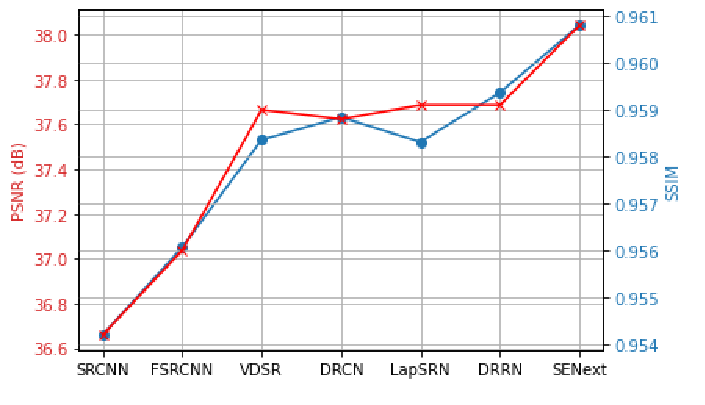
\includegraphics[width=\linewidth]{10FIGURE.pdf}
  \caption{Quantitative evaluation of average PSNR and SSIM of existing SR methods with an enlargement factor $\times2$.}
  \label{fig:10}
\end{figure}


\begin{figure}[ht]
  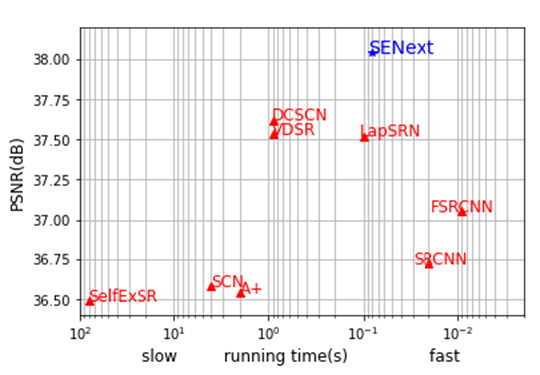
\includegraphics[width=\linewidth]{11FIGURE.pdf}
  \caption{Quantitative evaluations of PSNR versus running time on Set5 with enlargement factor $\times2$.}
  \label{fig:11}
\end{figure}



\subsection{Quantitative Analysis of run time versus PSNR}
In this section, we assess our SENext model's performance in terms of runtime time versus PSNR, as seen in Figure 11. To assess the state-of-the-art approaches using an Intel CPU i7-9750H having 2.60 GHz with supported card of NVIDIA GeForce RTX 2070 GPU (16 GB Memory). For evaluation purposes, we used the GitHub codes provided by the researchers. The trade-off between CPU time of execution versus PSNR on Set5 [60] enlargement factor $\times 2$ is present in Figure 11. Our proposed method is faster than recent state-of-the-art methods except then shallow models (SRCNN and FSRCNN). Furthermore, our proposed SENext attains less computation cost regarding floating point operations (FLOPs), as shown in Figure 12.

\begin{figure}[ht]
  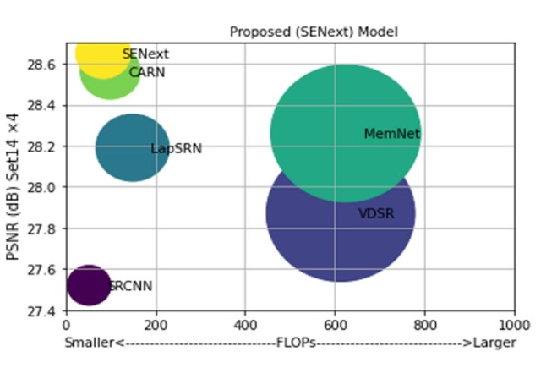
\includegraphics[width=\linewidth]{12FIGURE.pdf}
  \caption{Quantitative evaluations of PSNR versus FLOPs on Set14 enlargement factor $\times4$.}
  \label{fig:12}
\end{figure}





\subsection{Perceptual Quality Comparison}
Figure 13, 14, 15, 16, and 17 shows the perceptual quality of enlargement factor $\times 4$ and $\times 8$ image SR test datasets including BSDS100 [58], Urban100 [62] and Manga109 [63]. The results on challenging enlargement scale factor $\times 8$ observed that more blurry results were generated by Bicubic, RFL [5], SelfExSR [62], SRCNN [6], and FSRCNN [7]. However, it is a difficult effort to improve an image for an enlargement factor of $\times 8$. Our SENext successfully recovers the fine texture detail and effectively suppresses the artifacts.

The size of SqueezeNet [51] is extremely compact for mobile applications and has only 1.2 million parameters but achieves an accuracy similar to AlexNet [64]. During the design of SqueezeNet, the architecture used 26 convolution neural network layers without a fully-connected layer. SqueezeNet achieves a top-1 accuracy of 57.4\% and a top-5 accuracy of 80.5\% on ImageNet [64]. The potential applications of SqueezeNet   techniques are various in the field of image and computer vision tasks. The main versatile application of SqueezeNet is healthcare [65] and self-driving cars [67], where compact and efficient models are highly desirable. Self-driving cars rely heavily on real-time object detection to safely navigate through their environment. SqueezeNet has been used to improve the efficiency and accuracy of object detection in self-driving cars by quickly identifying objects such as pedestrians, cars, and traffic signs while consuming minimal computational resources [66]. Another major application of SqueezeNet used is in the field of medical imaging, where real-time image processing and diagnosis has been utilized to increase the effectiveness of medical imaging systems, including computed tomography (CT) and magnetic resonance imaging (MRI) scanners [67]. Quick CT image analysis and diagnosis can lead to better patient care and treatment results. Furthermore, face-mask detection [68] is also a central application of SqueezeNet to resolve the critical problems in security, surveillance, and healthcare. Finally, overall summary of state-of-the-art deep learning-based image SR methods present in Table 2.


\begin{table*}
\caption{Overall summary of state-of-the-art deep learning-based image SR methods.}

\label{table1}
\setlength{\tabcolsep}{4.5 pt}

\begin{tabular}{|c|c|c|c|c|c|c|c|c|c|c|c|c|c|}
\hline
Methods & LR & Bicubic & $\times 2$ & $\times 3$ & $\times 4$ & Parameters & Set5 & Set14 & BSDS100 & Urban100 & Manga109 & Loss & Optimizer\\

\hline

SRCNN [6] & $\times$  &  \checkmark & \checkmark  & \checkmark &\checkmark  & 57K    &\checkmark & \checkmark& $\times$ & $\times$ & $\times$ &$\ell ~$\footnotesize \textsubscript{2} &SGD\\
\hline


FSRCNN [7] & \checkmark &  $\times$ & \checkmark & \checkmark &\checkmark  &12K &\checkmark & \checkmark& $\times$ & $\times$ &$\times$& $\ell ~$\footnotesize \textsubscript{2} &SGD\\
\hline

VDSR [9] &  $\times$ &  \checkmark & \checkmark & \checkmark &\checkmark  &665K &\checkmark & \checkmark&\checkmark &\checkmark &$\times$& $\ell ~$\footnotesize \textsubscript{2}&SGD\\
\hline

DRCN [11] & $\times$ &  \checkmark & \checkmark & \checkmark &\checkmark  &1,774K &\checkmark & \checkmark&\checkmark &\checkmark &$\times$&$\ell ~$\footnotesize \textsubscript{2}&SGD\\
\hline


DRRN [24] & $\times$ &  \checkmark & \checkmark & \checkmark &\checkmark  &297K &\checkmark & \checkmark&\checkmark &\checkmark &$\times$&$\ell ~$\footnotesize \textsubscript{2}&SGD\\
\hline


MemNet [28] & $\times$ &  \checkmark & \checkmark & \checkmark &\checkmark  &677K &\checkmark & \checkmark&\checkmark &\checkmark &$\times$&$\ell ~$\footnotesize \textsubscript{2}&SGD\\
\hline

IDN [40] & \checkmark &  $\times$ & \checkmark & \checkmark &\checkmark  & 553K&\checkmark & \checkmark&\checkmark &\checkmark & \checkmark &$\ell ~$\footnotesize \textsubscript{1}, $\ell ~$\footnotesize \textsubscript{2}&Adam\\
\hline

SRMDNF [34] & \checkmark &  $\times$& \checkmark & \checkmark &\checkmark  & 1,511K &\checkmark & \checkmark&\checkmark &\checkmark & \checkmark &$\ell ~$\footnotesize \textsubscript{2}&Adam\\
\hline

MFEN\texttt{\_}S  [47] & \checkmark &  $\times$ & \checkmark & \checkmark &\checkmark  & 755K &\checkmark & \checkmark&\checkmark &\checkmark &\checkmark &$\ell ~$\footnotesize \textsubscript{1}&Adam\\
\hline


CARN [32] & \checkmark &  $\times$ & \checkmark & \checkmark &\checkmark  & 1,592K &\checkmark & \checkmark&\checkmark &\checkmark &$\times$&$\ell ~$\footnotesize \textsubscript{1}&Adam\\
\hline

IMDN [40] & \checkmark &  $\times$ & \checkmark & \checkmark &\checkmark  & 694K &\checkmark & \checkmark&\checkmark &\checkmark & \checkmark  &$\ell ~$\footnotesize \textsubscript{2}&Adam\\
\hline

\end{tabular}
\end{table*}



\begin{figure*}
    \centering

    \includegraphics[width=\linewidth]{13Figure.png}
    \caption{Visual perceptual quality-wise improvement of image 21077 obtained from BSDS100 dataset with $\times4$ enlargement factor.}
    \label{fig:13}
\end{figure*}



\begin{figure*}
    \centering

    \includegraphics[width=\linewidth]{14Figure.png}
    \caption{Visual perceptual quality-wise improvement of image 87046 obtained from BSDS100 dataset with $\times4$ enlargement factor.}
    \label{fig:14}
\end{figure*}

\begin{figure*}
    \centering

    \includegraphics[width=\linewidth]{15Figure.png}
    \caption{Visual perceptual quality-wise improvement of image 050 obtained from Urban100 dataset with $\times4$ enlargement factor.}
    \label{fig:15}
\end{figure*}


\begin{figure*}
    \centering

    \includegraphics[width=\linewidth]{16Figure.png}
    \caption{Visual perceptual quality-wise improvement of img060 image from Urban100 image test dataset with $\times8$ enlargement factor.}
    \label{fig:16}
\end{figure*}


\begin{figure*}
    \centering

    \includegraphics[width=\linewidth]{17Figure.png}
    \caption{Visual perceptual quality-wise improvement of MAD\texttt{\_}STONE image from Manga109 image test dataset with $\times8$ enlargement factor.}
    \label{fig:16}
\end{figure*}




\subsection{Ablation study}

\subsubsection{Model Analysis with Shallow Feature Extraction Block}
Design of a shallow feature extraction block as a backbone of deep CNN model. In this ablation study we compare a results of a model with a shallow feature extraction block and without shallow feature extraction. For quantitative ablation study purposes, we have trained two models separately, such as the SENext model with and without SFEB. Both models are trained on the same specification of GPU discussed in Section IV. For training purposes, we used only the Yang91 [1] image dataset. The quantitative experiment performs on benchmark test datasets such as Set5, Set14, BSDS00, Urban100 and Manga109 with enlargement factor $\times 4$  as shown in Table 3. Results in Table 3 clearly shows that a model with SFEB achieves better performance as compared to without SFEB. 

\begin{table}
\caption{Quantitative evaluations with and without SFEB on enlargement factor $\times4$.}
\label{table1}
\setlength{\tabcolsep}{3pt}
\centering
\begin{tabular}{|c|c|c|c|c|}
%\hline
%Scale       & Scale & \multicolumn{8}{c|}{Dataset}                                   \\
\hline
Scale         & Dataset & SFEB & PSNR (dB) & Parameters\\

\hline
$\times4$        & Set5 & $\times$  & 29.79 & 52K\\
\hline
$\times4$        & Set5 & \checkmark  & 30.37 & 54K\\
\hline


$\times4$        & Set14 & $\times$  & 27.99 & 52K\\
\hline
$\times4$        & Set14 & \checkmark  & 28.31 & 54K\\
\hline


$\times4$        & BSDS100 & $\times$  & 28.61 & 52K\\
\hline
$\times4$        & BSDS100 & \checkmark  & 28.91 & 54K\\
\hline

$\times4$        & Urban100 & $\times$  & 25.89 & 52K\\
\hline
$\times4$        & Urban100 & \checkmark  & 26.14 & 54K\\
\hline

$\times4$        & Manga109 & $\times$  & 26.65 & 52K\\
\hline
$\times4$        & Manga109 & \checkmark  & 26.99 & 54K\\
\hline

\end{tabular}
\end{table}



\subsubsection{Model Analysis with different Block arrangements}
A more comprehensive ablation study of our proposed blocks can be found in Table 4. In this experiment, we investigated the effects of various combinations of blocks. The eight networks were trained for super-resolution application with enlargement factor $\times 4$ and have the same configuration of training as well as validation parameters.  We used the 100 images of a DIV2K [27] dataset for training and 91 images from Yang91 [1]  for validation with 16 batch sizes having 100 epochs. In Table 4 PSNR value is reported and observed that the baseline network (without any block) gives the lowest PSNR value (28.11 dB), but the best performance (28.48 dB) is observed when all blocks are used in the model.

\begin{table}
\caption{Ablation study of different blocks, including SFEB, SEB, and SCB. The quantitative value of average PSNR calculated on Set14 enlargement factor $\times4$  on 100 epochs.}
\label{table1}
\setlength{\tabcolsep}{3pt}
\centering
\begin{tabular}{|c|c|c|c|c|c|c|c|c|}
\hline
Blocks       & \multicolumn{8}{c|}{Combination of Blocks}                    \\
\hline
SFEB         & $\times$& \checkmark & $\times$ & \checkmark&$\times$ & \checkmark& $\times$ & \checkmark\\
\hline
SEB          &$\times$& $\times$&  \checkmark&  \checkmark & $\times$& $\times$ &  \checkmark&  \checkmark\\
\hline
SCB          &$\times$& $\times$ &$\times$ & $\times$& \checkmark& \checkmark & \checkmark&\checkmark\\
\hline
Average PSNR & 28.11 & 28.23 & 28.20 & 28.35 & 28.38 & 28.42 & 28.45 & 28.48  \\
\hline
\end{tabular}
\end{table}


\subsubsection{Model Analysis with Activation Function}
Maas \textit{et al.} [15] evaluated a variant of ReLU with a gradient more amenable to optimization, which leads to Leaky ReLU [1]. Most common problems facing ReLU activation function is a Dying ReLU, which resolve by LReLU. For this ablation study purpose, we trained a three different model, such a model used only ReLU activation function, and other two models used LReLU activation with different value of $\alpha$ . The value of $\alpha$ is non-zero value over the entire domain, which allows a small leakage to activate the dead neurons. In Figure 18 and 19 results shows that network with LReLU has a more quick convergence and help networks to train faster.  Furthermore, a model with LReLU having value of $\alpha=0.2$ is less loss and higher value of PSNR as compare to LReLU with $\alpha=0.5$ and ReLU activation functions.    


\begin{figure}[ht]
  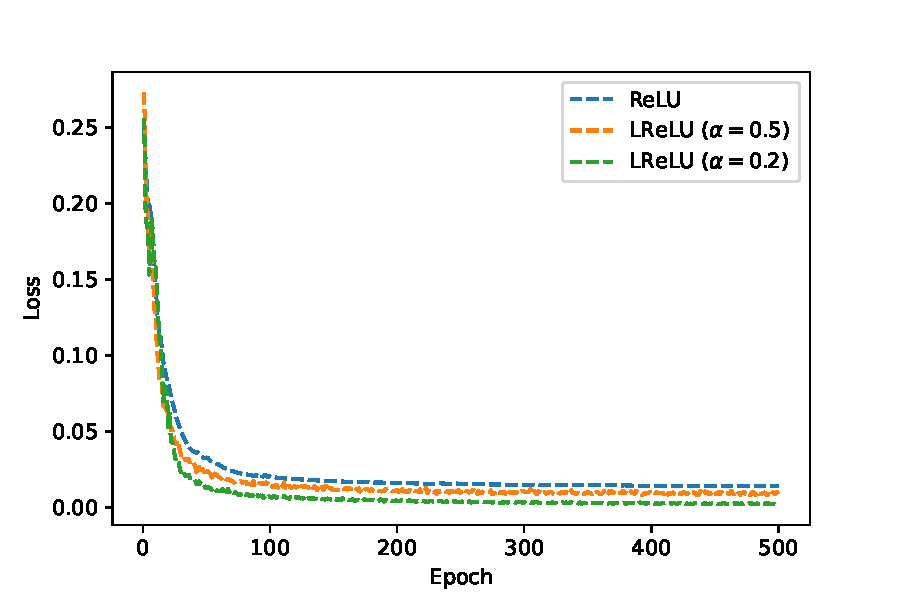
\includegraphics[width=\linewidth]{18FIGURE.pdf}
  \caption{Performance Analysis of loss versus epoch of activation functions.}
  \label{fig:17}
\end{figure}


\begin{figure}[ht]
  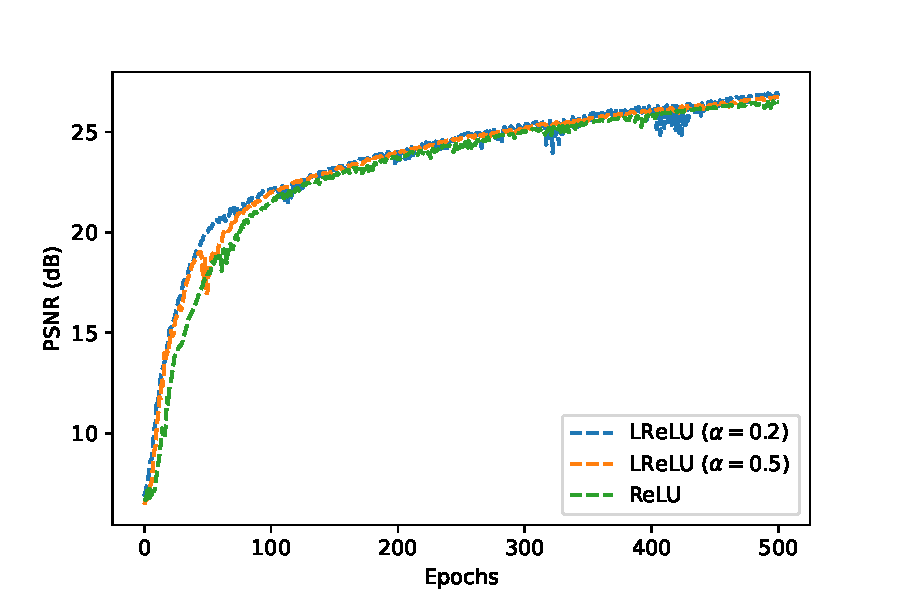
\includegraphics[width=\linewidth]{19FIGURE.pdf}
  \caption{Performance Analysis of PSNR (dB) versus epoch of activation functions.}
  \label{fig:17}
\end{figure}






\subsubsection{Model Analysis with Selection of Optimizers}
The selection of an optimizer plays a crucial role during the training to optimize the model efficiency and reduce the chance of overfitting. Our proposed SENext model is trained on four optimizers: Adam [69], Adamax, an enhanced version of Adam, and stochastic gradient descent (SGD). The experimental results with loss function as shown in Figure 20. Adam optimizer shows a more stable pattern as compare to other optimizers. RMSprop (green line) decreases slowly with more ripples after 400 iterations as compared to Adam. All optimizers were trained on 1000 epochs with the base model. Training images are obtained from a DIV2K (100 images) [27] dataset and Yang91 (91 images) [1]  images for validation with 16 batch sizes.

\begin{figure}[ht]
  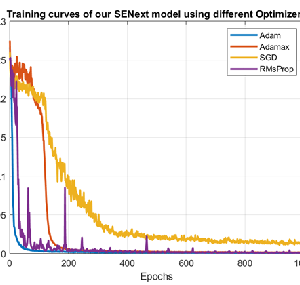
\includegraphics[width=\linewidth]{20FIGURE.pdf}
  \caption{Performance analysis for selection of Optimizers.}
  \label{fig:17}
\end{figure}



\subsubsection{Model Analysis in terms of Mean Inference Time}
The inference time is an important factor of image super-resolution methods other than the SR performance. In this part of ablation we shows the inference test time on publicly available datasets such as Set5, Set14, BSDS100, Urban100 and Manga109 with enlargement factor $2\times$, $3\times$, $4\times$ and $8\times$ as shown in Figure 21. Form the Figure 21, it is clearly seen that as the higher enlargement factor increasing the more processing time as compared to small scale factor, because input image having $2\times$ enlargement factor is higher than $8\times$ enlargement factor. Therefore, the computational cost of $2\times$ input image is higher than $8\times$ enlargement factor.

\begin{figure}[ht]
  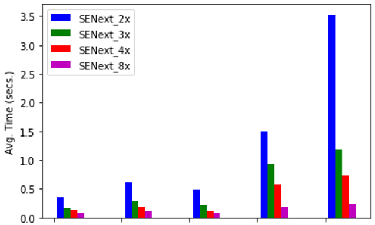
\includegraphics[width=\linewidth]{21FIGURE.pdf}
  \caption{Performance Analysis of Datasets (Number of Images) Versus Avergae Time on all test datasets.}
  \label{fig:21}
\end{figure}




\section{Conclusions and Future work}
In this study presents a novel two-stage squeeze (compress) and expanded method for Squeeze-and-ExcitationNext for Single Image Super-Resolution (SENext). Proposed SENext used SFEB, SEB, SCB, CUB, and UBB blocks with the support of local and global residual skip connection. The SFEB blocks are extract the low-frequency feature from the original LR an input image. The resultant new feature information are add to the remaining blocks through a long
and short skip paths. Implementation of SEB side-by-side reduces the computational cost of the network and calculates the high-frequency features information.
 The use of extensive sub-local skip connections helps to reduce vanishing gradient problems during the training. In addition, to activate the dead neurons in the model during the training, we replaced the conventional ReLU activation function with LReLU. Furthermore, the comparative analysis and ablation study shows the efficiency of a squeeze and excitation network to reduce lots of parameters and computational cost. Extensive evaluations on five benchmark test datasets showed that using a large upsampling factor of $\times 4$ or $\times 8$ improves the reconstruction results in both quantitative and qualitative criteria. In future, we will further optimize our model to introduce multi-path learning with dense global and local skip connections under complex scenarios.















\begin{thebibliography}{00}

\bibitem{b1} J. Yang, J. Wright, T. S. Huang and Y. Ma, "Image super-resolution via sparse representation", \textit{IEEE Trans. Image Process.}, vol. 19, no. 11, pp. 2861-2873, Nov. 2010.


\bibitem{b2} J. Yang, J. Wright, T. Huang and Y. Ma, "Image super-resolution as sparse representation of raw image patches", \textit{Proc. IEEE Conf. Comput. Vis. Pattern Recognit.}, pp. 1-8, Jun. 2008.


\bibitem{b3} C.-Y. Yang and M.-H. Yang, "Fast direct super-resolution by simple functions", \textit{Proc. IEEE Int. Conf. Comput. Vis.}, pp. 561-568, Dec. 2013.


\bibitem{b4} R. Timofte, V. De Smet and L. Van Gool, "A+: Adjusted anchored neighborhood regression for fast super-resolution", \textit{Proc. Asian Conf. Comput. Vis. (ACCV)}, pp. 111-126, 2014.


\bibitem{b5} S. Schulter, C. Lesistner and H. Bischof, "Fast and accurate image upscaling with super-resolution forests", \textit{Proc. IEEE Conf. Comput. Vis. Pattern Recognit.}, pp. 184-199, Jun. 2015.


\bibitem{b6} C. Dong, C. C. Loy, K. He and X. Tang, "Image super-resolution using deep convolutional networks", \textit{IEEE Trans. Pattern Anal. Mach. Intell.}, vol. 38, pp. 295-307, Feb. 2015.


\bibitem{b7} C. Dong, C. C. Loy and X. Tang, "Accelerating the super-resolution convolutional neural network", \textit{Proc. Eur. Conf. Comput. Vis.}, pp. 391-407, Oct. 2016.


\bibitem{b8} A. Krizhevsky, I. Sutskever and G. E. Hinton, "ImageNet classification with deep convolutional neural networks", \textit{Proc. Adv. Neural Inf. Process. Syst.}, pp. 1097-1105, 2012.


\bibitem{b9} J. Kim, J. K. Lee and K. M. Lee, "Accurate image super-resolution using very deep convolutional networks", \textit{Proc. IEEE Conf. Comput. Vis. Pattern Recognit.}, pp. 1646-1654, Jun. 2016.


\bibitem{b10} W. Shi, J. Caballero, F. Huszar, J. Totz, A. P. Aitken, R. Bishop, et al., "Real-time single image and video super-resolution using an efficient sub-pixel convolutional neural network", \textit{Proc. IEEE Conf. Comput. Vis. Pattern Recognit.}, pp. 1874-1883, Jun. 2016.



\bibitem{b11} J. Kim, J. K. Lee and K. M. Lee, "Deeply-recursive convolutional network for image super-resolution", \textit{Proc. IEEE Conf. Comput. Vis. Pattern Recognit.}, pp. 1637-1645, Jun. 2016.


\bibitem{b12} S. Anwar, S. Khan and N. Barnes, "A deep journey into super-resolution: A survey", \textit{ACM Comput. Surveys}, vol. 53, no. 3, pp. 1-34, May 2021.


\bibitem{b13} J. Hu, L. Shen and G. Sun, "Squeeze-and-excitation networks", \textit{Proc. Conf. Comput. Vis. Pattern Recognit. (CVPR)}, pp. 7132-7141, 2018.


\bibitem{b14} X. Cheng, X. Li, J. Yang and Y. Tai, "SESR: Single image super resolution with recursive squeeze and excitation networks", \textit{Proc. 24th Int. Conf. Pattern Recognit. (ICPR)}, pp. 147-152, Aug. 2018


\bibitem{b15} A. L. Maas, A. Y. Hannun and A. Y. Ng, "Rectifier nonlinearities improve neural network acoustic models", \textit{Proc. 30th Int. Conf. Mach. Learn.}, vol. 28, pp. 6, 2013.


\bibitem{b16} K. He, X. Zhang, S. Ren and J. Sun, "Delving deep into rectifiers: Surpassing human-level performance on ImageNet classification", \textit{Proc. IEEE Int. Conf. Comput. Vis}., pp. 1026-1034, Dec. 2015.



\bibitem{b17} Z. Wang et al., "Deep networks for image super-resolution with sparse prior", \textit{Proc. IEEE Int. Conf. Comput. Vis.}, pp. 370-378, 2015.


\bibitem{b18} Z. Wang, D. Liu, Z. Wang, J. Yang and T. Huang, "Deeply improved sparse coding for image super-resolution", \textit{Proc. IEEE Int. Conf. Comput. Vis.}, pp. 370-378, Dec. 2015.


\bibitem{b19} X. Mao, C. Shen and Y.-B. Yang, "Image restoration using very deep convolutional encoder-decoder networks with symmetric skip connections", In \textit{NIPS}, pp. 2802-2810, 2016.



\bibitem{b20} Y. Romano, J. Isidoro and P. Milanfar, "RAISR: Rapid and accurate image super resolution",\textit{IEEE Trans. Comput. Imag.}, vol. 3, no. 1, pp. 110-125, Oct. 2017.


\bibitem{b21} W.-S. Lai, J.-B. Huang, N. Ahuja and M.-H. Yang, "Deep Laplacian pyramid networks for fast and accurate super-resolution", \textit{Proc. IEEE Conf. Comput. Vis. Pattern Recognit.}, pp. 5835-5843, Jul. 2017.


\bibitem{b22} K. Zhang, W. Zuo, Y. Chen, D. Meng and L. Zhang, "Beyond a Gaussian Denoiser: Residual learning of deep CNN for image denoising", \textit{IEEE Trans. Image Process.}, vol. 26, no. 7, pp. 3142-3155, Jul. 2017.


\bibitem{b23} H. Zheng, G. Xinbo, Y.Yunchu and W. Xiumei, "Lightweight image super-resolution with information multidistillation network", \textit{Proc. of the ACM International Conference on Multimedia.}, pp. 2024-2032, 2019.


\bibitem{b24} Y. Tai, J. Yang and X. Liu, "Image super-resolution via deep recursive residual network", \textit{Proc. IEEE Conf. Comput. Vis. Pattern Recognit.}, pp. 2790-2798, Jul. 2017.



\bibitem{b25} C. Ledig et al., "Photo-realistic single image super-resolution using a generative adversarial network", \textit{Proc. IEEE Conf. Comput. Vis. Pattern Recognit. (CVPR)}, pp. 105-114, Jul. 2017.


\bibitem{b26} B. Lim, S. Son, H. Kim, S. Nah and K. M. Lee, "Enhanced deep residual networks for single image super-resolution", \textit{Proc. IEEE Conf. Comput. Vis. Pattern Recognit. Workshops}, pp. 136-144, Jul. 2017.


\bibitem{b27} E. Agustsson, and R. Timofte, "NTIRE 2017 challenge on single image super-resolution: Dataset and study",\textit{Proc. IEEE Conf. Comput. Vis. Pattern Recognit. Workshops}, pp. 126-135, Jul. 2017.


\bibitem{b28} Y. Tai, J. Yang, X. Liu and C. Xu, "MemNet: A persistent memory network for image restoration", \textit{Proc. IEEE Conf. Int. Conf. Comput. Vis.}, pp. 4539-4547, Oct. 2017.


\bibitem{b29} J. Yamanaka, S. Kuwashima and T. Kurita, "Fast and accurate image super resolution by deep cnn with skip connection and network in network", \textit{Proc. ICNIP}, pp. 217-225, 2017.


\bibitem{b30} W. Han, S. Chang, D. Liu, M. Yu, M. Witbrock and T. S. Huang, "Image super-resolution via dual-state recurrent networks", \textit{Proc. IEEE/CVF Conf. Comput. Vis. Pattern Recognit.}, pp. 1654-1663, Jun. 2018.


\bibitem{b31} J. Li, F. Fang, K. Mei and G. Zhang, "Multi-scale residual network for image super-resolution", \textit{Proc. Eur. Conf. Comput. Vis. (ECCV)}, pp. 517-532, Sep. 2018.


\bibitem{b32} N. Ahn, B. Kang and K.-A. Sohn, "Fast accurate and lightweight super-resolution with cascading residual network", \textit{ Proceedings of the European conference on computer vision (ECCV)}, pp. 252-268, 2018.


\bibitem{b33} J.-H. Choi, J.-H. Kim, M. Cheon and J.-S. Lee, "Lightweight and efficient image super-resolution with block state-based recursive network",\textit{arXiv:1811.12546} , 2018, [online] Available: http://arxiv.org/abs/1811.12546.


\bibitem{b34} K. Zhang, W. Zuo and L. Zhang, "Learning a single convolutional super-resolution network for multiple degradations", \textit{Proc. IEEE/CVF Conf. Comput. Vis. Pattern Recognit.}, vol. 6, no. 1, pp. 3262-3271, Jun. 2018.


\bibitem{b35} W. Muhammad, and S. Aramvith, "Multi-scale inception based super-resolution using deep learning approach",\textit{Electronics}, vol. 8, no.8, pp.892, 2019.


\bibitem{b36}R. Wang, M. Gong and D. Tao, "Receptive field size versus model depth for single image super-resolution", \textit{IEEE Trans. Image Process.}, vol. 29, pp. 1669-1682, 2019.


\bibitem{b37} Y. Wang, L. Wang, H. Wang and P. Li, "End-to-end image super-resolution via deep and shallow convolutional networks", \textit{IEEE Access}, vol. 7, pp. 31959-31970, Mar. 2019.


\bibitem{b38} X. Yang, H. Mei, J. Zhang, K. Xu, B. Yin, Q. Zhang, et al., "DRFN: Deep recurrent fusion network for single-image super-resolution with large factors", \textit{IEEE Trans. Multimedia}, vol. 21, no. 2, pp. 328-337, Feb. 2019.


\bibitem{b39} M. Su, S. Lai, Z. Chai, X. Wei, and Y. Liu, "Hierarchical Recursive Network for Single Image Super Resolution",\textit{IEEE International Conference on Multimedia \& Expo Workshops (ICMEW)}, pp. 595-598, 2019.


\bibitem{b40} Z. Hui, X. Wang and X. Gao, "Fast and accurate single image super-resolution via information distillation network", \textit{Proc. IEEE/CVF Conf. Comput. Vis. Pattern Recognit.}, pp. 723-731, Jun. 2018.


\bibitem{b41} K.-W. Hung, Z. Zhang and J. Jiang, "Real-time image super-resolution using recursive depthwise separable convolution network", \textit{IEEE Access}, vol. 7, pp. 99804-99816, 2019.



\bibitem{b42}S. Barzegar, A. Sharifi, and M. Manthouri, "Super-resolution using lightweight detailnet network", \textit{Multimedia Tools and Applications}, vol. 79, pp.1119-1136, 2020


\bibitem{b43} W. Muhammad, S. Aramvith, and T. Onoye, "Multi-scale Xception based depthwise separable convolution for single image super-resolution", \textit{Plos one} vol.16, no. 8, pp. e0249278, 2021.



\bibitem{b44} J.-T. Hsu, C.-H. Kuo and D.-W. Chen, "Image super-resolution using capsule neural networks", \textit{IEEE Access}, vol. 8, pp. 9751-9759, 2020.



\bibitem{b45} B. Liu and D. Ait-Boudaoud, "Effective image super resolution via hierarchical convolutional neural network", \textit{Neurocomputing}, vol. 374, pp. 109-116, Jan. 2020.



\bibitem{b46} J. Cheng, W. Wang, T. Liu, Z. Zhang, and H. Gao, “A POCS super resolution restoration algorithm based on BM3D”, \textit{Sci. Rep.}, vol. 7, 2017, Art. no. 15049.


\bibitem{b47} H. Xiao, J. Qin, S. Jeon, B. Yan, and X. Yang "MFEN: Lightweight multi-scale feature extraction super-resolution network in embedded system", \textit{Microprocessors and Microsystems}, vol. 93, pp.104568, 2022.


\bibitem{b48} J. Qin, R. Zhang, " Lightweight single image super-resolution with attentive residual refinement network", \text{Neurocomputing}, 500, pp.846-855 , 2022.


\bibitem{b49}J.Li, F. Fang, T. Zeng, G. Zhang, and X. Wang, "Adjustable super-resolution network via deep supervised learning and progressive self-distillation", \textit{Neurocomputing}, vol. 500, pp.379-393, 2022.



\bibitem{b50} Y. Zhang, K. Li, K. Li, L. Wang, B. Zhong and Y. Fu, "Image super-resolution using very deep residual channel attention networks",\textit{Proc. Eur. Conf. Comput. Vis.}, pp. 286-301, Sep. 2018.



\bibitem{b51} F. N. Iandola, S. Han, M. W. Moskewicz, K. Ashraf, W. J. Dally and K. Keutzer, " SqueezeNet: AlexNet-level accuracy with $50\times$ fewer parameters and < 0.5 MB model size " in \textit{arXiv:1602.07360}, 2016,
[online] Available: https://arxiv.org/abs/1602.07360.


\bibitem{b52} K. He, X. Zhang, S. Ren and J. Sun, "Deep residual learning for image recognition", \textit{Proc. IEEE Conf. Comput. Vis. Pattern Recognit.}, pp. 770-778, Jun. 2016.


\bibitem{b53} K. Chang, M. Li, P. L. K. Ding and B. Li, "Accurate single image super-resolution using multi-path wide-activated residual network",  \textit{Signal Process.}, vol. 172, Jul. 2020.


\bibitem{b54} Y. Zhou, Y. Zhang, X. Xie and S.-Y. Kung, "Image super-resolution based on dense convolutional auto-encoder blocks", \textit{Neurocomputing}, vol. 423, pp. 98-109, Jan. 2021.


\bibitem{b55} C. Szegedy et al., "Going deeper with convolutions", \textit{Proc. IEEE Conf. Comput. Vis. Pattern Recognit.}, pp. 1-9, Jun. 2015.


\bibitem{b56} R. Nirthika,"Pooling in convolutional neural networks for medical image analysis: a survey and an empirical study." \textit{Neural Computing and Applications}, vol. 34, no. 7, pp.  5321-5347.


\bibitem{b57} S. Sabour, N. Frosst and G. E. Hinton, "Dynamic routing between capsules", \textit{Proc. Adv. Neural Inf. Process. Syst.}, pp. 3859-3869, 2017.


\bibitem{b58} P. Arbelaez, M. Maire, C. Fowlkes and J. Malik, "Contour detection and hierarchical image segmentation", \textit {IEEE Trans. Pattern Anal. Mach. Intell.}, vol. 33, no. 5, pp. 898-916, May 2011.


\bibitem{b59} F. Li, H. Bai, and Y. Zhao, ‘‘Detail-preserving image super-resolution via recursively dilated residual network,’’ \textit {Neurocomputing}, vol. 358, pp. 285–293, Sep. 2019.


\bibitem{b60} M. Bevilacqua, A. Roumy, C. Guillemot and M. L. Alberi-Morel, "Low-complexity single-image super-resolution based on nonnegative neighbor embedding", in\textit{Proc. Brit. Mach. Vis. Conf.,} pp. 1-10, 2012.

\bibitem{b61} R. Zeyde, M. Elad, and M. Protter, ‘‘On single image scale-up using sparse-representations,’’ in \textit {Proc. Int. Conf. curves Surf}. Berlin, Germany: Springer, 2010, pp. 711–730.


\bibitem{b62} J.-B. Huang, A. Singh, and N. Ahuja, “Single image super-resolution from transformed self-exemplars,” in \textit {Proceedings of the IEEE conference on computer vision and pattern recognition}, 2015, pp. 5197–5206.


\bibitem{b63} Y. Matsui, K. Ito, Y. Aramaki, A. Fujimoto, T. Ogawa, T. Yamasaki, and K. Aizawa, ‘‘Sketch-based Manga retrieval using Manga109 dataset,’’ \textit {Multimedia Tools Appl.}, vol. 76, no. 20, pp. 21811–21838, 2017.



\bibitem{b64} A. Krizhevsky, I. Sutskever, and G. E. Hinton, “ImageNet classification with deep convolutional neural networks” \textit{ Proc. 26th Annu. Conf. Neural Inf. Process. Syst},  pp. 1097–1105, 2012.

\bibitem{b65} V. Kumar, and B. Bakariya, "Detection of Lung Malignancy Using SqueezeNet-Fc Deep Learning Classification Technique",  \textit{Proc. of the International Conference on Paradigms of Communication, Computing and Data Sciences: PCCDS }, pp. 683-699, 2021.
    
\bibitem{b66}  H. Lee, I. Ullah, W. Wan, Y. Gao, and Z. Fang, ‘‘Real-time vehicle make and model recognition with the residual SqueezeNet architecture,’’ \textit{Sensors}, vol. 19, no. 5, p. 982, Feb. 2019.

\bibitem{b67} M. Tsivgoulis, T. Papastergiou, and V. Megalooikonomou, "An improved SqueezeNet model for the diagnosis of lung cancer in CT scans" , \textit{Machine Learning with Applications}, p.100399

\bibitem{b68} O. P. Kwaghe, A. Y. Gital, A. G. Madaki, M. L. Abdulrahman, I. Z. Yakubu and I. S. Shima, “A Deep Learning Approach for Detecting Face Mask Using an Improved Yolo-V2 With Squeezenet,” \textit{2022 IEEE 6th Conference on Information and Communication Technology (CICT),} pp. 1–5, 2022. 

\bibitem{b69} D. Kingma and J. Ba, "Adam: A method for stochastic optimization", \textit {Proc. Int. Conf. Learn. Representations}, pp. 1-15, 2015.

\end{thebibliography}

\begin{IEEEbiography}[{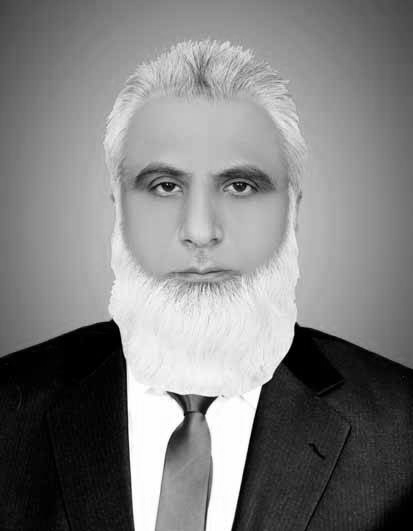
\includegraphics[width=1in,height=1.25in,clip,keepaspectratio]{a.png}}]{Wazir Muhammad} (Graduate Student Member, IEEE) received the B.E. in Electrical
Engineering and ME in Communication Systems \& Networks from Mehran University of Engineering and Technology, Jamshoro, Sindh, Pakistan in 1999 and 2007. Dr. Wazir received his doctoral degree from the Department of Electrical Engineering Chulalongkorn University Bangkok, Thailand in 2019. His research interests lie in the areas of Electrical Engineering, Communication Systems, Neural Networks, and Machine Learning, specifically in Deep Learning image super-resolution.

\end{IEEEbiography}

\begin{IEEEbiography}[{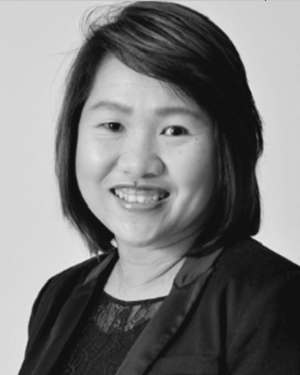
\includegraphics[width=1in,height=1.25in,clip,keepaspectratio]{b.png}}]{SUPAVADEE ARAMVITH} (Senior Member, IEEE) received the B.S. degree (Hons.) in computer science from Mahidol University, in 1993, and the M.S. and Ph.D. degrees in electrical engineering from the University of Washington, Seattle, USA, in 1996 and 2001, respectively. In June 2001, she joined Chulalongkorn University, where she is currently an Associate Professor at the Department of Electrical Engineering, with a specialization in video technology. She has successfully advised 32 bachelor’s, 27 master’s, and 10 Ph.D. graduates. She published over 130 articles in international conference proceedings and journals with four international book chapters. She has rich project management experiences as a project leader and a former technical committee chairs to the Thailand Government bodies in Telecommunications and ICT. She is very active in the international arena with the leadership positions in the international network, such as JICA Project for AUN/SEEDNet, and the professional organizations, such as the IEEE, IEICE, APSIPA, and ITU.
\end{IEEEbiography}

\begin{IEEEbiography}[{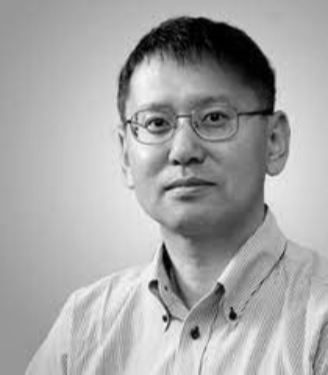
\includegraphics[width=1in,height=1.25in,clip,keepaspectratio]{c.png}}]{Takao Onoye} (Senior Member, IEEE) received the B.E. and M.E. degrees in electronic engineering and the Dr.Eng. degree in information systems engineering from Osaka University, Osaka, Japan, in 1991, 1993, and 1997, respectively.,He was an Associate Professor with the Department of Communications and Computer Engineering, Kyoto University, Kyoto, Japan. Since 2003, he has been a Professor with the Department of Information Systems Engineering, Osaka University. He has published over 200 research papers in the field of VLSI design and multimedia signal processing in reputed journals and proceedings of international conferences. His current research interests include media-centric low-power architecture and its SoC implementation.,Dr. Onoye has been served as a member of the CAS Society Board of Governors, since 2008. He is also a member of IEICE, IPSJ, and ITE-J.


\end{IEEEbiography}




\EOD

\end{document}
